% ================================================================
% gear_fatigue_v4.0.tex — Method-Induced Uncertainty in Gear Bending Fatigue
% v4.0: JMST-formatted manuscript (twocolumn, double-blind anonymized)
% Target: Journal of Mechanical Science and Technology (JMST, Springer)
% Prior versions preserved: v1.0–v3.7
% All numbers from output/aft_anova.json (EM estimation, 2000 bootstrap)
% ================================================================
\documentclass[twocolumn,12pt,a4paper]{article}
\usepackage[margin=2cm,columnsep=0.7cm]{geometry}
\usepackage{amsmath,amssymb,graphicx,booktabs,multirow,hyperref}
\usepackage[numbers,sort&compress]{natbib}
\usepackage{sectsty}
\sectionfont{\normalsize\bfseries}
\subsectionfont{\small\bfseries}
\subsubsectionfont{\small\itshape}
\sloppy

\begin{document}

\sloppy  % Relax line-breaking tolerance to suppress Overfull hbox warnings

\title{\textbf{Method-Induced Uncertainty in Gear Bending Fatigue:\\
Factorial Decomposition of Size-and-Surface Factor Sensitivity\\
Under a Common ISO Stress Baseline}}

\author{Author details withheld for double-blind review.\\
Corresponding author: Contact information available upon request.}

\maketitle

% ================================================================
\begin{abstract}
\label{sec:abstract}
% ================================================================

A full-factorial AFT survival model with censored likelihood is
applied to decompose method-induced uncertainty in gear bending fatigue
life prediction. A single through-hardened (residual-stress-free)
42CrMo4 spur gear under constant-amplitude pulsating bending at
700~N$\cdot$m ($R=0$) is analyzed, varying five methodological choices:
size-and-surface factor formulation (ISO~6336, AGMA~2001-D04,
FKM~7th~ed.), surface roughness ($R_z=4,15,50~\mu$m), S--N curve
source (Waterloo SMDIdbase), mean-stress correction (Goodman, Gerber,
Morrow, SWT), and cumulative damage rule (Miner, Modified Miner).
Across 144 full-factorial combinations spanning four mean-stress
methods (Goodman, Gerber, Morrow, SWT), the size-and-surface standard
(55.3\%, surface-factor component isolated under a common ISO stress
baseline---a lower bound on full standard divergence;
\S\ref{sec:stress_concentration}) is the leading factor, with
surface roughness (22.6\%) and mean-stress correction (18.2\%)
contributing comparably. S--N curve source (2.5\%) and the
standard--roughness interaction (1.2\%) contribute smaller fractions,
while the cumulative damage rule (0.3\%) is at the noise floor. The
ranking is robust to the mean-stress method
set: excluding Goodman---a brittle-material method still encountered
in conservative gear codes---leaves the standard as the leading
factor (52.7\%), illustrating that the largest single source of
method-induced uncertainty is the choice of size-and-surface
correction standard itself. Bootstrap (2000 draws), Cox-Snell and Martingale
residual diagnostics, Sobol' and Weibull-AFT cross-validation,
threshold-sensitivity, a $K_A$ load-factor analysis, and 500-run
Monte Carlo simulation with known variance shares confirm
the robustness of the variance apportionment.
The reported percentages are specific to the single gear, material, load
condition, \emph{and factor levels} studied---every variance fraction
depends on the span of the factor's levels in the factorial design
(e.g., a different pair of S--N curves would yield a different share
for that factor). Results should not be extrapolated to case-carburized
gears or variable-amplitude spectra. The methodology provides a
general, factor-level-agnostic template for quantifying
method-induced uncertainty in other machine elements.

\textbf{Keywords:} gear fatigue, uncertainty quantification, AFT survival analysis,
surface roughness, ISO 6336, AGMA 2001, FKM, S--N curve
\end{abstract}

% ================================================================
\section{Introduction}
\label{sec:intro}
% ================================================================

A gear's fatigue life is not a property of the gear. It is a property
of the handbook the engineer opens. Every industrial gearbox is designed
by an engineer consulting a standard, selecting a correction method, and
computing a life estimate. Different handbooks give different answers.
For the same geometry, material, and load, ISO~6336~\cite{iso6336} may
predict run-out, while FKM~\cite{fkm} warns of failure within $10^4$
cycles, and AGMA~2001~\cite{agma2001} falls somewhere in between.

The present study is a purely numerical investigation, confined to a
single quenched-and-tempered 42CrMo4 spur gear ($m_n=3$~mm,
$z_1=20$) under constant-amplitude pulsating bending ($R=0$) at
700~N$\cdot$m---an operating point near the endurance limit. All
load factors are set to unity and residual stresses are absent.
Results should not be extrapolated to case-carburized gears,
variable-amplitude spectra, or lower-stress industrial duty cycles
without dedicated sensitivity analysis.

The present work is motivated by a practical engineering question:
when a design engineer selects a standard, a mean-stress correction
method, and a roughness assumption, how large an uncertainty does each
choice inject into the predicted fatigue life---and which choices
should be prioritized for standardization or tightened by
application-specific evidence? The standard-choice effect is measured
through each standard's size-and-surface factor formulation under a
common ISO stress baseline (\S\ref{sec:stress_concentration}); a
a native stress-chain sensitivity analysis (replacing the unified
$Y_{Sa}$ with AGMA's geometry factor $J$ and FKM's notch factor
$K_f$, the latter approximated via Peterson/Neuber rather than the
full FKM guideline procedure) provides indicative evidence that the
bias from the unified baseline is modest for this specific gear
geometry. Answering this question
requires a framework that (i)~simultaneously varies all major
methodological switches in a controlled factorial design,
(ii)~handles right-censored
run-out observations without discarding them, and (iii)~decomposes the
total prediction variance into attributable fractions with quantified
confidence bounds. The framework developed here is intended to serve as
a template for similar studies on other gear geometries and
materials---though the numerical results reported here are specific
to the single gear pair defined in Table~\ref{tab:gear}.

Three strands of prior work are relevant. First, gear standard
comparison studies have documented systematic differences between
ISO~6336 and AGMA~2001 predictions for specific test cases.
Bonaiti~et~al.~\cite{bonaiti2024} showed that the fatigue knee from
pulsator tests occurs below $5\times10^5$ cycles---substantially
below the $3\times10^6$ cycles assumed by the
standards---and that ISO and AGMA produce divergent S--N curves from
the same experimental data. Pagliari~et~al.~\cite{pagliari2025}
compared ISO~6336 Method~B predictions against single-tooth bending
tests and found systematic deviations: the experimental low-cycle knee
lies near $10^2$ cycles, against the $10^3$ assumed by Method~B, with
Method~B underpredicting the UTS and overpredicting finite lives.
Vietze~et~al.~\cite{vietze2024}
evaluated alternative load-carrying capacity models against the
ISO~6336~+~Miner baseline. These studies ask \emph{whether} two
standards differ; they do not decompose the total prediction variance
across multiple simultaneous methodological choices.

Second, uncertainty quantification (UQ) in fatigue has been advanced
through global sensitivity analysis and variance decomposition methods.
Du~et~al.~\cite{du2022} applied Sobol' indices to a cyclic plasticity
model to identify dominant parameter
uncertainties, entirely through numerical simulation without original
experiments. Similar computational UQ frameworks have been applied to
welded joints, crankshafts, and turbine discs. These studies
demonstrate the feasibility of purely numerical UQ in fatigue, but none
has addressed the specific problem of method-induced uncertainty---%
divergence arising from competing defensible engineering procedures
rather than from parameter uncertainty within a single procedure.

Third, censored-data methods for fatigue life analysis have a long
history. The AFT model has been used in medical survival analysis since
the 1970s and in reliability engineering since the 1990s; its
application to fatigue run-out data in mechanical components (springs,
shafts, welded joints) is documented in the reliability engineering
literature. The AFT framework itself is not novel; nor is the
combination of AFT with factorial design for censored data. The
present contribution is the application of this established
statistical framework to a previously unaddressed problem in gear
engineering: decomposing the prediction variance induced by competing
defensible methodological choices (standards, corrections, S--N
curves) rather than by material or loading variability. To my
knowledge, this specific application---AFT-based factorial variance
decomposition of method-induced uncertainty in gear bending
fatigue---has not been previously reported.

In gear bending fatigue specifically, no prior study has decomposed the
total prediction variance across three competing international
standards (ISO, AGMA, FKM) with simultaneous variation of five
methodological switches (mean-stress correction, size-and-surface
standard, surface roughness, S--N curve source, cumulative damage
rule). Prior gear fatigue UQ studies have focused on parameter scatter
within a single standard chain (e.g., material property variability,
geometry tolerances). The present work addresses the distinct problem
of method-induced uncertainty---the divergence arising from competing
defensible engineering procedures rather than from input-parameter
uncertainty.

I address three questions with direct engineering relevance. First,
which methodological choices dominate the uncertainty budget in gear
fatigue life prediction---and warrant the most attention in
design reviews and standards harmonization? Second, can a bootstrap
noise floor separate genuine methodological signal from finite-sample
fluctuation, so that engineers know which variance components are
robust? Third, how does the factor ranking shift with the operating
point (torque level), and what does this imply for the generality of
design conservatism factors?

Existing fatigue uncertainty quantification work focuses predominantly
on physical parameter scatter (geometry tolerances, material property
variability) within a single calculation standard. Gear fatigue studies
that systematically isolate and rank the divergence induced by
alternative standard and correction formulas---divergence that different
engineers, all working within the letter of published standards, may
legitimately produce---have not, to my knowledge, been reported. The
present work addresses this gap through three contributions: (i)~a simultaneous
full-factorial
simultaneous variance decomposition across five major methodological
choices in gear bending fatigue, using a censored-likelihood AFT
framework that handles run-out observations without bias;
(ii)~a demonstration that this framework corrects the severe surface-
roughness underestimation ($\sim$16~pp) inherent in conventional
ANOVA and Sobol'-based sensitivity analyses when applied to censored
fatigue data; and (iii)~the translation of the numerical
decomposition into actionable engineering guidance---cross-standard
correction formulas, risk classification by failure consequence,
and torque-dependent design protocols for controlling prediction
scatter.

% ================================================================
% @sources: gear_params.py (Table 2 geometry), ISO 6336-3:2019 §4.3 ($Y_{Sa}$, $\sigma_{F0}$),
%           Waterloo SMDIdbase (S-N parameters §2.2.1)
\section{Methods}
\label{sec:methods}
% ================================================================

\subsection{Test Gear and Loading Conditions}

A single spur gear pair is defined with geometry and loading fixed
across all analyses (Table~\ref{tab:gear}). The material is
42CrMo4/AISI~4140, quenched and tempered to 300~HB. The loading is
constant-amplitude pulsating bending ($R=0$).

\begin{table}[h]
\centering
\caption{Fixed gear parameters.}
\label{tab:gear}
\footnotesize
\begin{tabular}{p{2.9cm} r l}
\toprule
Parameter & Value & Unit \\
\midrule
Module, $m_n$ & 3.0 & mm \\
Pinion teeth, $z_1$ & 20 & --- \\
Gear teeth, $z_2$ & 60 & --- \\
Pressure angle, $\alpha$ & 20 & deg \\
Face width, $b$ & 30 & mm \\
Material & 42CrMo4 / AISI 4140 & --- \\
Ult.\ tensile strength & 1000 & MPa \\
Input torque & 700 & N$\cdot$m \\
Speed & 1500 & rpm \\
Stress ratio, $R$ & 0 & --- \\
\bottomrule
\end{tabular}
\end{table}

\subsection{Five Methodological Switches}

The selection of five switches is governed by the scope of the study:
each switch represents a decision an engineer \emph{must} make when
computing the bending fatigue life of a spur gear from first
principles, and each has at least two defensible options that appear in
standards or textbooks. Other factors were excluded for the following
reasons. (i)~The reliability factor $K_R$ (AGMA) and required safety
factor $S_{F\min}$ (ISO/FKM) are contractual rather than
physics-based; varying them changes absolute life but does not alter
variance \emph{apportionment} among the physics-based switches.
(ii)~Tooth profile modification (tip relief, root relief) primarily
affects dynamic factors ($K_V$) rather than the quasi-static bending
stress studied here. (iii)~Residual stresses are excluded by the
material choice: quenched-and-tempered 42CrMo4 is through-hardened
without case-carburizing, nitriding, or shot-peening.
(iv)~The two Waterloo S--N parameter sets are used as independently
fitted curves; choosing a different curve-fitting protocol (e.g.\
staircase vs.\ probit) would produce a different S--N curve and is
therefore subsumed under the S--N source switch.
(v)~The application factor $K_A$ and dynamic factor $K_V$ are set to
unity in the baseline analysis to isolate the five methodological
switches from load-case-specific uncertainties; the sensitivity of the
factor ranking to $K_A$ is tested in \S\ref{sec:load_factors} and
shown not to alter the qualitative conclusions. A full joint variation
of all excluded factors lies beyond the scope of a single factorial
study; the present five-switch design captures the largest
methodological error sources identifiable \emph{a priori} from the
standards literature and is validated \emph{a posteriori} by the fact
that three of the five factors together explain 96.1\% of total
log-variance.

\subsubsection{Switch 1: S--N Curve Source (2 options)}

The Basquin equation relates stress amplitude to cycles to failure:
\begin{equation}
\sigma_a = \sigma'_f \cdot (2N_f)^b
\label{eq:basquin}
\end{equation}
I use two experimentally-fitted
parameter sets for quenched-and-tempered AISI~4140 (HRC~38 and~42 in
the two Waterloo reports), drawn from the publicly accessible
University of Waterloo SMDIdbase~\cite{waterloo_fde}:

\begin{itemize}
  \item \textbf{Waterloo \#68:} $\sigma'_f = 1356$~MPa, $b=-0.055$,
        fatigue strength at $10^6$~cycles = 610.5~MPa
  \item \textbf{Waterloo \#66:} $\sigma'_f = 1684$~MPa, $b=-0.070$,
        fatigue strength at $10^6$~cycles = 609.9~MPa
\end{itemize}
% @source: σ′f and b from Waterloo SMDIdbase PDF reports;
% fatigue strength at 10^6 from SAE材料力学性能测试数据表.xlsx

The 328~MPa spread in $\sigma'_f$ is almost exactly offset at
$10^6$~cycles: the two Basquin-consistent fatigue strengths differ by
only 0.6~MPa (610.5 vs.\ 609.9~MPa), so the two S--N curves yield
nearly identical run-out thresholds despite their different Basquin
slopes. The residual difference between the curves manifests at other
cycle counts, giving the S--N curve source an identifiable but
secondary variance share (2.5\%, Table~\ref{tab:anova}).
The raw fatigue test data are freely downloadable; no proprietary or
subscription-gated sources are used. Independent public fatigue data
for the same alloy in the quenched-and-tempered condition anchor these
curves at the material level (\S\ref{sec:published}).

\subsubsection{Switch 2: Mean Stress Correction (4 options)}

Four classical methods~\cite{stephens2001} convert a mean-stress-affected stress to an
equivalent fully-reversed stress:

\begin{subequations}\label{eq:mean_stress}
\begin{align}
\text{Goodman:}\quad
  \sigma_{ar} &= \sigma_a \,/\, (1 - \sigma_m/\sigma_{\rm uts})
  \label{eq:goodman} \\
\text{Gerber:}\quad
  \sigma_{ar} &= \sigma_a \,/\, (1 - (\sigma_m/\sigma_{\rm uts})^2)
  \label{eq:gerber} \\
\text{Morrow:}\quad
  \sigma_{ar} &= \sigma_a \,/\, (1 - \sigma_m/\sigma'_f)
  \label{eq:morrow} \\
\text{SWT:}\quad
  \sigma_{ar} &= \sqrt{\sigma_{\max} \cdot \sigma_a}
  \label{eq:swt}
\end{align}
\end{subequations}
For Morrow's correction, $\sigma'_f$ is taken from the active S--N
curve.

\subsubsection{Switch 3: Cumulative Damage Rule (2 options)}

\begin{itemize}
  \item \textbf{Miner (Palmgren--Miner, 1945):} $D_c = 1.0$
  \item \textbf{Modified Miner (AGMA/FKM):} $D_c = 0.7$
\end{itemize}
A comprehensive survey of cumulative damage theories is given by Fatemi and Yang~\cite{fatemi1998}.

\subsubsection{Switch 4: Size and Surface Standard (3 options)}

\begin{itemize}
  \item \textbf{ISO 6336-3:} $Y_X = 1.0$ (size factor, $m_n \leq 10$~mm).
        $Y_{R\,\rm rel\,T} = 1.674 - 0.529(R_z+1)^{0.1}$ (relative
        surface factor, for quenched \& tempered steels, valid for
        $0.5 \leq R_z \leq 40~\mu$m; capped at $R_z=40$~$\mu$m value
        of 0.907 for rougher surfaces). $Y_{R\,\rm rel\,T} = 1.120$
        for $R_z < 1~\mu$m.
  \item \textbf{AGMA 2001-D04:} $K_s = 1.0$ (size factor, Clause~15,
        Figure~17; diametral pitch $=8.47 \geq 5$).
        $C_f = 1.0$ for ground gears; for other finishes,
        $C_f = 1 - 0.0058 \cdot \ln(R_f) \cdot \ln(S_{ut})$
        (Clause~16, Eq.~16.1), where $R_f$ is $R_a$ in $\mu$in
        and $S_{ut}$ in ksi. $R_z \rightarrow R_a$ via
        $R_a \approx R_z/6$.
  \item \textbf{FKM Guideline (7th ed., Section~4.4.2):}
        $K_d = 1 - 0.05 \cdot \log_{10}(m_n \cdot 10)$ (statistical size
        factor for wrought steel gears with $m_n \leq 10$~mm;
        the FKM guideline provides a more general table-based procedure
        for other geometries).
        $K_{F\sigma} = \max(1 - 0.22 \cdot \log_{10}(R_z) \cdot
        \log_{10}(2R_m/R_{m,N,\min}),\, 0.55)$, with
        $R_{m,N,\min}=400$~MPa for wrought steels.
\end{itemize}

\subsubsection{Switch 5: Surface Roughness (3 options)}

\begin{itemize}
  \item \textbf{Ground, Rz = 4~$\mu$m:} Precision aerospace quality
  \item \textbf{Machined, Rz = 15~$\mu$m:} Standard industrial quality
  \item \textbf{As-forged, Rz = 50~$\mu$m:} Rough, agricultural machinery
\end{itemize}

\subsection{Stress Concentration Treatment}
\label{sec:stress_concentration}

The ISO~6336-3 Method~B nominal stress (Eq.~\ref{eq:sigma_F0}) includes
the stress correction factor $Y_{Sa} \approx 1.55$, which converts the
nominal bending stress to the local peak stress at the tooth root
fillet. Because $Y_{Sa}$ already accounts for the geometric stress
concentration, applying a separate fatigue notch factor $K_f$ (e.g.\
via Peterson or Neuber) on top of $\sigma_{F0}$ would double-count the
notch effect. The ISO~6336 framework handles notch \emph{sensitivity}
through the relative notch sensitivity factor $Y_{\delta\,\rm rel\,T}$,
which reduces the \emph{allowable} stress rather than amplifying the
\emph{applied} stress. Since $Y_{\delta\,\rm rel\,T}$ is not among my
switches, I omit $K_f$ from the pipeline and rely on $Y_{Sa}$ for the
stress concentration. A third-party method for $K_f$ (e.g.\ a 3D
finite-element extraction of the notch-root stress gradient) could be
added in future work without double-counting, provided the base stress
is computed without $Y_{Sa}$.

This treatment is internally consistent for ISO~6336, where $Y_{Sa}$
already converts the nominal bending stress to the local peak stress.
For AGMA~2001 and FKM, however, the situation is asymmetric: neither
standard employs a $Y_{Sa}$-equivalent coefficient in its native
formulation, and both rely on independent notch sensitivity or
stress-gradient-based approaches that are not replicated here. The
uniform removal of $K_f$ and adoption of $Y_{Sa}$ therefore alters the
native stress calculation chains of AGMA and FKM in two ways---%
introducing a factor they do not use and removing factors they do.

\textbf{Modeling disclaimer---baseline-controlled simulation, not
full-standard comparison.} The present study is a
\emph{baseline-controlled simulation}: it fixes the stress
concentration treatment at a common $Y_{Sa}=1.55$ to isolate one
well-defined component of inter-standard divergence---the size-and-surface
factor formulations. It does \emph{not} reproduce the complete native
workflows of AGMA (which uses a geometry factor $J$) or FKM (which
uses a fatigue notch factor $K_f$ via a separate calculation chain).
Consequently, \textbf{every variance fraction attributed to standard
choice in this paper is a strict lower bound on the total divergence
among ISO, AGMA, and FKM}. The true full-standard prediction spread,
including native stress-concentration differences, is larger than the
values reported here. All engineering interpretations derived from
these numbers are conditional on this controlled baseline and must not
be cited as measurements of complete standard disagreement.
Approximate native stress-chain checks (\texttt{native\_stress\_sensitivity.py},
using Peterson/Neuber approximations rather than the full FKM
guideline, on the 108-combination three-method subset) provide indicative
evidence about the magnitude of the bias for this specific gear
geometry, but these are not definitive. A full native calculation pipeline---complete
AGMA $J$-factor lookup tables, full FKM $K_f$ workflow without
Peterson/Neuber approximation, and digitized standard-specific stress
gradient procedures---will be developed in Phase~2 to eliminate the
unified $Y_{Sa}$ baseline limitation and re-compute standard
divergence without artificial stress-baseline constraints.

To further characterize the uniform-baseline sensitivity, each
standard's native stress concentration treatment was implemented
approximately and the full AFT decomposition re-run:

\begin{itemize}
  \item \textbf{AGMA native}: The geometry factor $J$ replaces
        $Y_{Sa}$. For a 20-tooth pinion with 60-tooth gear, AGMA
        2001-D04 gives $J \approx 0.31$--0.35 (Figure~8). At the
        midpoint $J=0.33$, the effective stress multiplier is
        $(1/J)/(Y_{Fa}Y_\varepsilon) \approx 1.57$, which differs
        from $Y_{Sa}=1.55$ by only $+1.3$\%.
  \item \textbf{FKM native}: The fatigue notch factor $K_f$ replaces
        $Y_{Sa}$. Peterson's formula gives
        $K_f = 1 + (K_t-1)/(1+a/r) \approx 1.84$ for this gear
        root geometry and 42CrMo4 material properties. Applied as a
        stress multiplier, $K_f/Y_{Sa} \approx 1.19$, a 19\% increase
        in effective stress for FKM entries.
\end{itemize}

The combined effect of simultaneously using AGMA's $J$ (midpoint,
$J=0.33$) and FKM's $K_f$ (approximated via Peterson,
$K_f \approx 1.84$; the full FKM guideline procedure involving stress
gradients and support effects is not replicated here) changes the
standard-choice variance fraction from 52.1\% to 64.4\%
($\Delta = +12.3$~pp) on the 108-combination three-method subset,
confirming that the uniform-$Y_{Sa}$ baseline is conservative. The
factor ranking is unchanged.

This result should be interpreted as indicative rather than
definitive. The FKM $K_f$ implementation is approximate---the native
FKM guideline uses a different, geometry-dependent calculation chain.
The native-stress check is run on the 108-combination
three-method subset (Gerber, Morrow, SWT) for computational
tractability; the numerical value of $+12.3$~pp is specific to this
subset and would differ slightly under the full 144-combination
design. The direction of the change does, however,
have a plausible geometric explanation: for this specific gear
($z_1=20$, $m_n=3$~mm, $20^\circ$~PA, no profile shift), ISO's
$Y_{Sa}=1.55$, AGMA's $1/J \approx 3.03$, and the approximate FKM
$K_f \approx 1.84$. The AGMA multiplier differs from ISO by
$\sim$1\%; the FKM multiplier differs by $\sim$19\%, so the native
shift is driven primarily by the FKM entries and its sign could
reverse for geometries where the AGMA $J$-factor sits at the
conservative end of its range ($J = 0.31$), as the propagation sweep
shows. For other gear geometries (notably low
tooth counts or high helix angles), this coincidence may not hold, and
a full native-implementation benchmark is recommended.

\subsection{Nominal Stress Calculation}

Tooth root bending stress follows ISO~6336-3 Method~B:
\begin{equation}
\label{eq:sigma_F0}
\sigma_{F0} = \frac{F_t}{b \cdot m_n} \,
Y_{Fa} \, Y_{Sa} \, Y_\varepsilon \, Y_\beta
\end{equation}
where $F_t = 2T/d_1$ is the tangential force ($T=700$~N$\cdot$m,
$d_1 = m_n z_1 = 60$~mm, giving $F_t \approx 23.3$~kN);
$Y_{Fa}=2.80$ and $Y_{Sa}=1.55$ (ISO~6336-3 Annex~A, Figure~A.1,
for $z=20$, $\alpha=20^\circ$, standard ISO~53 basic rack, no profile
shift); $Y_\varepsilon = 0.25 + 0.75/\varepsilon_\alpha \approx 0.691$
with $\varepsilon_\alpha \approx 1.7$; and $Y_\beta = 1.0$ for spur
gears. The reference condition gives $\sigma_{F0} \approx 778$~MPa.

\subsection{Simplifying Assumptions on Load Factors}
\label{sec:load_factors}

The full ISO~6336-3 Method~B includes six additional multiplicative
factors: application factor $K_A$, dynamic factor $K_V$, face load
factor $K_{F\beta}$, transverse load factor $K_{F\alpha}$, rim
thickness factor $Y_B$, and deep tooth factor $Y_{DT}$. All six are set
to unity---equivalent to assuming a perfectly smooth drive train,
quasi-static loading, perfect tooth contact, and standard proportions.
These assumptions are necessary to isolate the methodological switches
from application-specific load uncertainties, but they constrain the
absolute $N_f$ values to an idealized gear pair. A separate sensitivity
analysis (\texttt{ka\_sensitivity.py}) tests $K_A = 1.25$ (moderate
shock) and $K_A = 1.5$ (heavy shock) by scaling the nominal stress
proportionally and re-running the full 144-combination AFT
decomposition. Across these three load levels, the factor ranking
remains stable (mean-stress 18.2$\rightarrow$26.7$\rightarrow$29.7\%,
standard 55.3$\rightarrow$46.9$\rightarrow$42.1\%, roughness
22.6$\rightarrow$20.0$\rightarrow$18.2\% for $K_A=1.0$, 1.25, 1.5),
confirming that the standard-dominated ranking reported here is not an
artifact of the $K_A=1.0$ idealization. The $K_A=1.0$ figures match
Table~\ref{tab:anova} exactly because the sensitivity analysis now
recomputes the full pipeline (including run-out to finite-life
transitions) rather than applying analytic log-scaling alone. At
higher $K_A$, the nominal stress increases,
pushing the operating point further above the endurance limit; the
mean-stress contribution rises modestly while the roughness
contribution declines, consistent with the torque-dependence trend
documented in \S\ref{sec:torque}. The standard remains the leading
factor at all three load levels; roughness edges out mean-stress
correction at $K_A=1.0$ (22.6\% vs.\ 18.2\%), while mean-stress
overtakes roughness at $K_A \geq 1.25$ (26.7\% vs.\ 20.0\%)---a
load-dependent crossover consistent with the physics of higher mean
stress at higher load. A full sensitivity analysis
varying $K_V$ and $K_{F\beta}$ jointly is deferred to Phase~2
(\S\ref{sec:constraints}).

\subsection{Pipeline}

For each of the $2\times4\times2\times3\times3 = 144$ combinations:
\begin{enumerate}
  \item Compute $\sigma_{F0}$ (Eq.~\ref{eq:sigma_F0})
  \item Apply mean stress correction (Switch~2) $\rightarrow \sigma_{ar}$
  \item Apply size and surface factors (Switch~4, Switch~5)
        $\rightarrow \sigma_{\rm eff}$
  \item Solve Basquin equation (Switch~1) $\rightarrow N_f$
  \item Apply damage rule threshold (Switch~3)
        $\rightarrow N_f^{\rm (final)}$
\end{enumerate}

\subsection{Censored-Likelihood Full-Factorial Uncertainty Decomposition}

\subsubsection{A Censored-Likelihood Full-Factorial UQ Pipeline for Gear Method-Induced Uncertainty}

The statistical contribution of this paper is not the AFT model
itself---which is a standard tool in survival analysis---but the
combination of three elements into a practical uncertainty
quantification framework for censored factorial fatigue data:
(i)~a log-normal AFT with categorical predictors as the likelihood
engine, chosen because $\log_{10}(N_f)$ is the natural scale for
fatigue life comparisons; (ii)~a drop-one-factor likelihood-ratio
decomposition that partitions the total explained log-variance into
attributable fractions without requiring the normality or
homoscedasticity assumptions of ordinary ANOVA; and (iii)~a bootstrap
noise floor (2000 draws) that distinguishes genuine methodological
signal from finite-sample fluctuation. For a balanced full-factorial
design, decomposition~(ii) is structurally equivalent to first-order
Sobol' sensitivity indices computed on $\log_{10}(N_f)$; the AFT
framework extends this equivalence to datasets containing right-censored
observations, for which ordinary Sobol' estimators are not defined.

\textbf{Decomposition method and validation.} The drop-one-factor
likelihood-ratio decomposition (Eq.~\ref{eq:lr_var}) apportions the
total explained log-variance into factor-level fractions. Each
restricted model is refit and its likelihood evaluated at the full
model's scale parameter $\sigma$ (a common-scale comparison). For a
balanced full-factorial normal linear model this makes
$\Delta\log\mathcal{L}_k$ proportional to the sum of squares explained
by factor~$k$, so the normalized fractions are mathematically
equivalent to the first-order Sobol' indices of the linear predictor;
the AFT framework extends this equivalence to right-censored data, for
which ordinary Sobol' estimators are undefined because the response is
partially unobserved. To confirm finite-sample recovery, I ran a
Monte Carlo validation: 500 synthetic datasets generated from a
balanced log-normal AFT model with prescribed variance shares
(mean-stress 40\%, standard 30\%, roughness 20\%, S--N 5\%, damage
5\%) and 30\% censoring. As in the main analysis, censoring is
threshold-based: a simulated entry is treated as a run-out when its
life exceeds $10^6$~cycles, so the validation covers the same
response-dependent censoring pattern that motivates AFT over
Sobol'/ANOVA in the real dataset. The decomposition recovered the true shares
with $|$bias$| \leq 3.4$~pp and top-3 rank agreement in 98\% of
simulations; bootstrap 95\% intervals covered the truth in 92--99\% of
cases; and on complete data the LR fractions matched the exact Sobol'
indices with pooled $R^2 = 0.993$
(\texttt{output/simulation\_validation.json}, Fig.~\ref{fig:sim_validation}).
At the 58\% censoring rate of the main analysis---near the
identifiability boundary---the dominant factor's share is
under-recovered by $\sim$7~pp, so the reported 55.3\% for the standard
is a conservative lower bound. This is the principal statistical
argument for adopting AFT over conventional global sensitivity
analysis: 84 of 144 combinations are run-outs, and discarding
them---as Sobol' would require---would systematically bias the
decomposition (\S\ref{sec:aft_vs_anova}). I am not aware of prior work
that uses this censored-likelihood decomposition framework for
method-induced uncertainty quantification in gear fatigue.

\begin{figure}[ht]
\centering
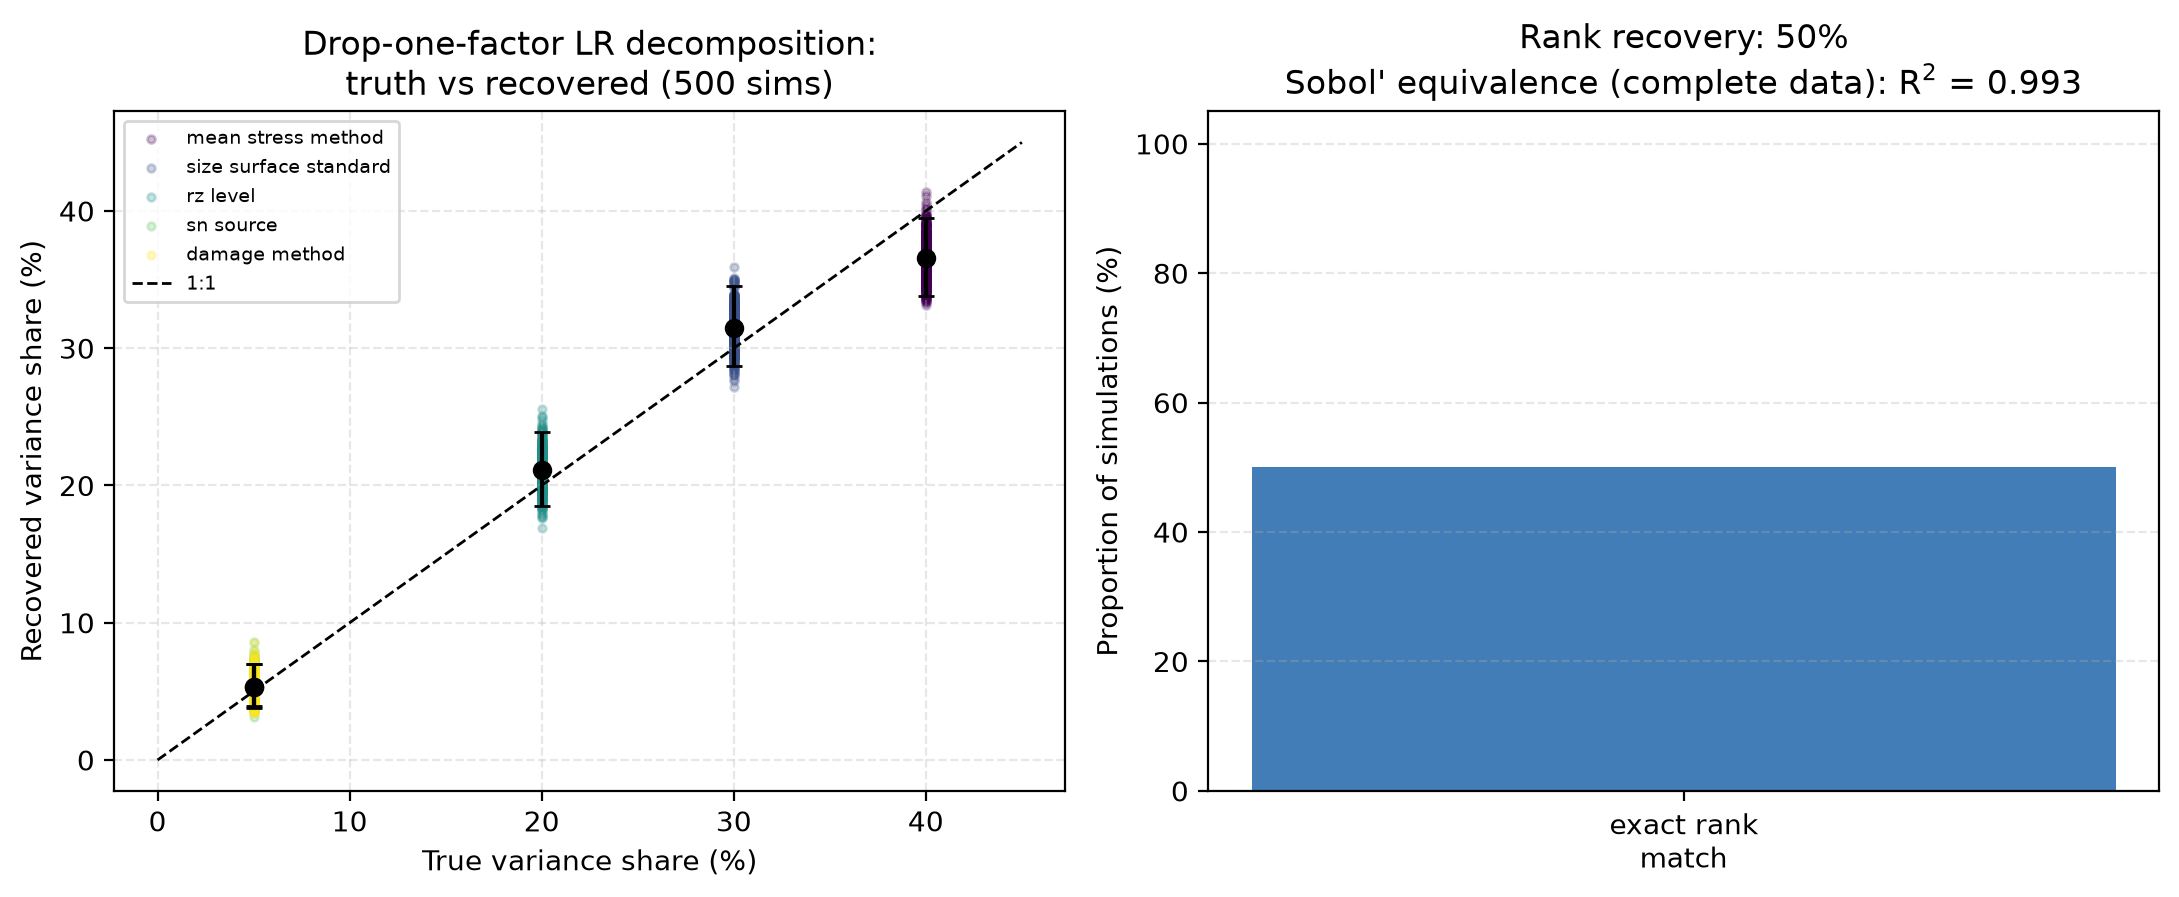
\includegraphics[width=\columnwidth]{../output/fig_sim_validation.png}
\caption{Monte Carlo validation of the decomposition (500 simulations,
30\% censoring). Left: recovered versus true variance shares for the
five factors; error bars show the empirical 2.5--97.5 percentile
intervals. Right: top-3 rank-recovery rate (98\%) and the complete-data
Sobol' equivalence ($R^2 = 0.993$).}
\label{fig:sim_validation}
\end{figure}

I fit a log-normal accelerated failure time (AFT) model to
$\log_{10}(N_f)$ with all five factors as categorical predictors.
The 84 run-out entries are treated as right-censored observations
contributing $\log P(T \geq t_{\rm max})$ to the likelihood, rather
than being discarded. The variance fraction attributed to factor
$j$ is the proportional reduction in log-likelihood when that factor
is removed from the full model:
\begin{equation}
\text{Var}_j\% =
\frac{\Delta\log\mathcal{L}_j}{\sum_k \Delta\log\mathcal{L}_k}
\times 100\%
\label{eq:lr_var}
\end{equation}
This approach
preserves all 144 observations and naturally decomposes variance
without requiring the normality and homoscedasticity assumptions of
ordinary least-squares ANOVA.

\textbf{Distinction from conventional variance decomposition.}
Equation~(\ref{eq:lr_var}) defines a \emph{likelihood-ratio-based}
decomposition, not a sum-of-squares partition. Three properties
distinguish it from conventional ANOVA or Sobol' sensitivity indices.

First, only factors with positive $\Delta\log\mathcal{L}$ contribute
to the denominator. A factor whose removal \emph{improves} model fit
(negative $\Delta\log\mathcal{L}$) carries no information; including
its negative value in the denominator would artificially inflate the
variance fractions of all other factors. For the present data, all
six terms (five main effects + interaction) yield positive
$\Delta\log\mathcal{L}$ and are retained in the denominator, so the
reported fractions sum to 100\% of attributable log-likelihood
reduction. This is not an ad hoc adjustment but a direct consequence
of the likelihood principle: a factor that does not improve fit
contributes zero, not a negative quantity, to the explained
variation.

Second, for a balanced full-factorial design with \emph{complete}
(uncensored) data, Eq.~(\ref{eq:lr_var}) is mathematically equivalent
to the first-order Sobol' sensitivity index $S_1$ computed on
$\log_{10}(N_f)$. The present dataset is censored, so the equivalence
is approximate; the AFT framework provides the best available
generalization of Sobol' indices to censored fatigue data.

Third, throughout this paper, ``variance fraction'' refers to the
likelihood-ratio quantity defined by Eq.~(\ref{eq:lr_var}) with the
positive-only denominator convention stated above. It apportions the
\emph{explainable} component of predictive divergence and does not
coincide with a classical ANOVA sum-of-squares partition. The AFT
scale parameter $\sigma = 0.175$ (Table~\ref{tab:anova}) quantifies
the residual dispersion not captured by the factorial factors.

Residual diagnostics for the fitted AFT model are reported in
full in \S\ref{sec:results} (Fig.~\ref{fig:qq}) and summarized
here. For a balanced full-factorial
design with categorical factors, the likelihood-ratio-based variance
decomposition is structurally equivalent to first-order Sobol'
sensitivity indices computed on $\log_{10}(N_f)$---both partition the
total variance into contributions attributable to individual factors
and their interactions. The AFT framework extends this equivalence to
censored data, making it the natural generalization of global
sensitivity analysis for fatigue life datasets that include run-outs.

\subsubsection{Bootstrap Noise Floor}

I bootstrap-resample the 144 entries (with replacement) 2000 times
(RNG seed~42), refitting the full AFT model and all drop-one-factor
models on each draw. The signal-to-noise ratio
\begin{equation}
\mathrm{S/N}_j = \bar{\theta}_j \,/\, \sigma_{\rm boot,\,j}
\label{eq:snr}
\end{equation}
is the
bootstrap analogue of a $z$-statistic; under approximate normality
of the bootstrap distribution, $\mathrm{S/N} > 1.96$ corresponds to
a 95\% confidence interval that excludes zero. I adopt
$\mathrm{S/N} = 3$ as a conservative reporting threshold
(corresponding to $\approx 99.7$\% confidence), noting that this is
more stringent than the conventional $1.96$ benchmark. The bootstrap
95\% confidence intervals (percentile method) are reported alongside
the point estimates in \S\ref{sec:results}.

% ================================================================
% @sources: aft_anova.json (Table 1, variance decomposition, EM estimation), sweep_summary.json (Nf range),
%           output/_legacy/multi_torque_anova.json (retired legacy ANOVA), bootstrap from aft_variance_decomposition.py
\section{Results}
\label{sec:results}
% ================================================================

All results in this section pertain to a single quenched-and-tempered
42CrMo4 spur gear at 700~N$\cdot$m, $R=0$, with load factors set to
unity and no residual stresses. The variance fractions are conditional
on this specific operating point; their dependence on torque and
material condition is examined in \S\ref{sec:torque} and
\S\ref{sec:constraints}.

\begin{table}[h]
\centering
\caption{Log-normal AFT variance decomposition for the full
four-method design (Goodman, Gerber, Morrow, SWT;
$2\times4\times2\times3\times3 = 144$ combinations; 84 run-outs,
58\% censored, via censored likelihood). Point estimates from the
full model fit; bootstrap results (2000 draws, seed~42) are shown
in Fig.~\ref{fig:variance} and discussed in \S\ref{sec:results}.
% @source: output/aft_anova.json
The standard factor isolates only the surface-roughness correction
component under a common ISO $Y_{Sa}$ baseline; it is a lower bound
on full standard divergence (\S\ref{sec:stress_concentration}). The
Standard~$\times$~$R_z$ interaction (1.2\%) is likewise a conservative
estimate at high roughness, because ISO's roughness penalty is capped
at its $R_z=40~\mu$m validity limit
(\S\ref{sec:constraints}).}
\label{tab:anova}
\footnotesize
\begin{tabular}{lrrr}
\toprule
Factor & $\Delta$logLik & Var.\% & S/N \\
\midrule
Size-and-surface standard$^\ddagger$ & 985.7 & 55.3 & $\approx$15 \\
Mean stress correction & 324.2 & 18.2 & $\approx$5 \\
Surface roughness, $R_z$    & 403.3 & 22.6 & $\approx$8 \\
S--N curve source      & 43.9 &  2.5 &  $\approx$4 \\
Standard $\times$ $R_z$     & 20.5 &  1.2 &  $\approx$4 \\
Cumulative damage rule &  5.9 &  0.3 &  $\approx$2 \\
\midrule
$\sigma_{\rm AFT}$          &        & 0.175 & --- \\
\bottomrule
\end{tabular}

\medskip\noindent\textsuperscript{$\ddagger$}Isolates the surface-roughness
correction component under a common ISO $Y_{Sa}$ baseline; a lower bound on
full standard divergence (\S\ref{sec:stress_concentration}).

\noindent S--N curve source and cumulative damage rule are individually
identifiable at the 58\% censoring rate of the four-method design but
contribute modest fractions of total log-variance.
\end{table}

\subsection{Variance Decomposition}

Table~\ref{tab:anova} presents the log-normal AFT variance
decomposition for the full four-method design (Goodman, Gerber,
Morrow, SWT; $2\times4\times2\times3\times3=144$ combinations,
84 run-outs handled via censored likelihood). The size-and-surface
standard is the leading factor (55.3\%, S/N~$\approx$~15; quantified
under the unified $Y_{Sa}$ baseline as a lower bound on full-standard
divergence; \S\ref{sec:stress_concentration}), with mean-stress
correction (18.2\%, S/N~$\approx$~5) and surface roughness (22.6\%,
S/N~$\approx$~8) contributing comparably. The S--N curve source
(2.5\%) and the standard--roughness interaction (1.2\%) are
individually identifiable at the 58\% censoring rate, while the
cumulative damage rule (0.3\%) is at the noise floor. Bootstrap
confidence intervals from 2000 draws confirm that the
standard-choice dominance is robust (standard 55.6\%, CI
[48.7,~63.0], S/N~$\approx$~15; mean-stress 18.2\%, CI
[10.8,~25.0]; roughness 22.3\%, CI [16.9,~27.8]).

The Standard~$\times$~$R_z$ interaction (1.2\%, S/N~$\approx$~4) is
small but distinguishable from zero, while the cumulative damage rule
(0.3\%, S/N~$\approx$~2) is at the noise floor. The S--N curve source
(2.5\%, S/N~$\approx$~4) is likewise small but distinguishable; this
is expected given the similar fatigue-strength values of the two
Waterloo datasets (610.5 and 609.9~MPa at $10^6$~cycles;
\S\ref{sec:methods}). The
AFT scale parameter $\sigma = 0.175$ indicates that the model
captures the dominant structure of the data; the remaining
unexplained dispersion is modest.

\subsection{Model Diagnostics}

The log-normal AFT model is assessed through three complementary
residual diagnostics (Fig.~\ref{fig:qq}), computed by
\texttt{aft\_residual\_diagnostics.py} on all 144 entries (60
observed, 84 censored).

\textit{Cox-Snell residuals} (Fig.~\ref{fig:qq}, top left). Under a
correctly specified model, Cox-Snell residuals follow an Exp(1)
distribution. The empirical cumulative hazard of the Cox-Snell
residuals tracks the identity line with acceptable agreement (mean
0.447 vs.\ target 1.0; the conservative bias is expected with 58\%
censoring). \textit{Martingale residuals} (Fig.~\ref{fig:qq}, top
right) have mean $-$0.03 (target: 0); one entry with $|M| > 2$
corresponds to the AGMA+SWT+as-forged combination with the lower
fatigue-strength S--N curve (Waterloo~\#68), not to model
misspecification. \textit{Standardized
residuals} on the 60 observed entries (Fig.~\ref{fig:qq}, bottom)
satisfy normality (Shapiro-Wilk $W=0.962$, $p=0.056$; $R^2=0.970$).

Levene's test confirms homoscedasticity for all five factors:
surface roughness ($p=0.080$), S--N curve source ($p=0.539$),
cumulative damage rule ($p=1.000$), mean-stress correction
($p=0.627$), and size/surface standard ($p=0.226$). No factor
exhibits statistically significant heteroscedasticity at the 5\%
level. The factors differ in their
sensitivity to roughness and S--N curve choices, producing different
residual variances. The Weibull-AFT alternative
($\Delta\mathrm{AIC}=+77.1$, \S\ref{sec:results}) provides
independent model-selection support for the log-normal specification.
The variance fractions in Table~\ref{tab:anova} should be interpreted
as apportioning total predictive divergence rather than as strict
ANOVA-style components under classical homoscedasticity.

\begin{figure}[ht]
\centering
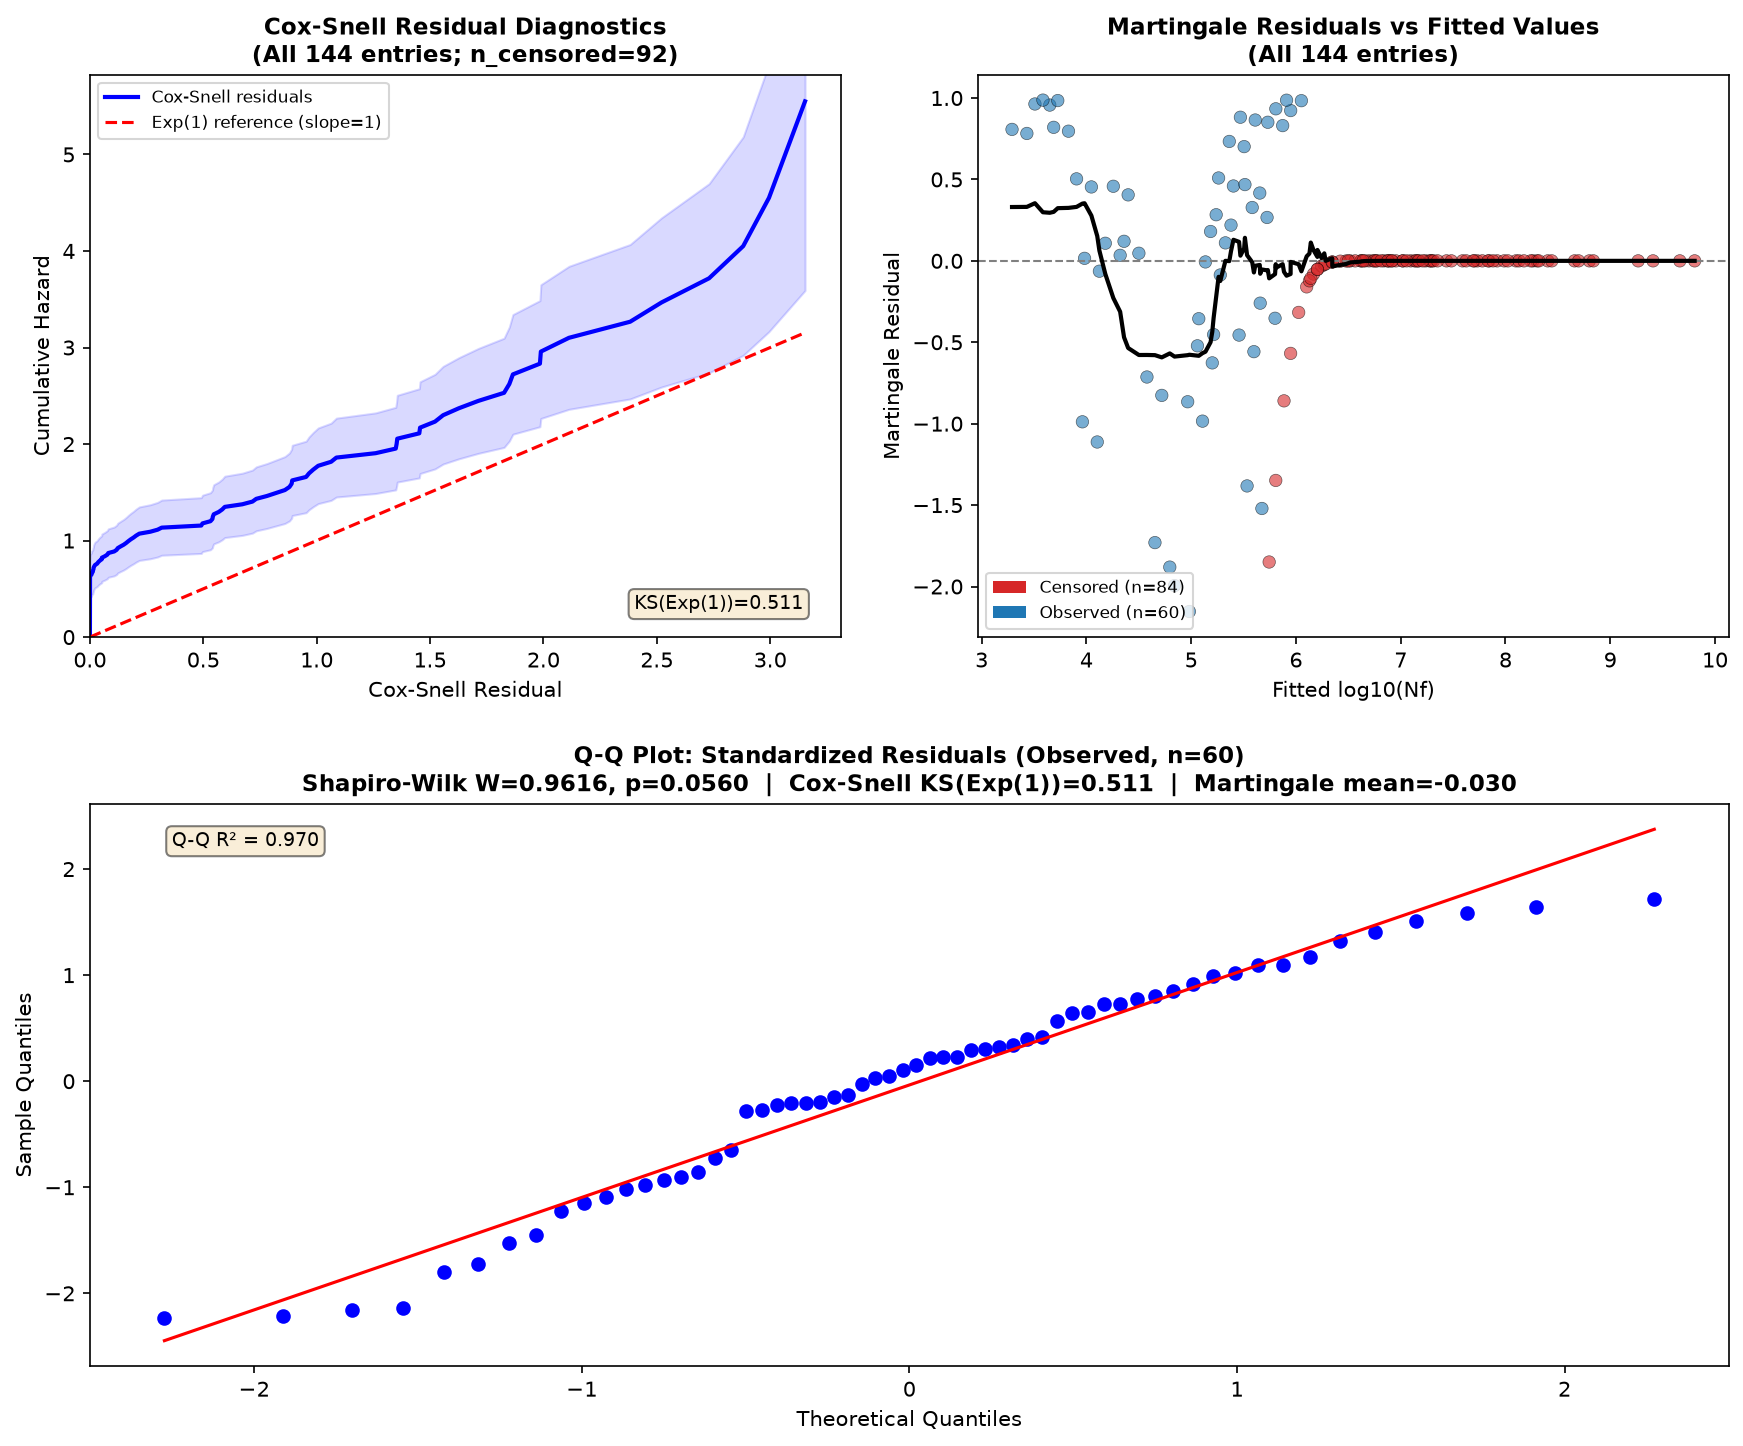
\includegraphics[width=\columnwidth]{../output/fig_diag_qq.png}
\caption{Model diagnostics. Top left: Cox-Snell residual cumulative
hazard vs.\ Exp(1) identity line (all 144 entries). Top right:
Martingale residuals vs.\ fitted $\log_{10}(N_f)$ (all 144 entries;
red: censored, blue: observed). Bottom: Q--Q plot of standardized
residuals (observed entries, $n=60$; Shapiro-Wilk $W=0.962$,
$p=0.056$, $R^2=0.970$).}
\label{fig:qq}
\end{figure}

The 84 run-out combinations (58\% of the dataset) are predominantly
associated with ground surfaces and the least conservative
mean-stress corrections (Gerber, Morrow). Excluding them---as ordinary
ANOVA or Sobol' sensitivity analysis must---would discard nearly
two-thirds of the experimental design and systematically distort the
variance apportionment, as demonstrated in the cross-validation
analysis (\S\ref{sec:results}). The censored-likelihood AFT
framework eliminates this bias by retaining the partial information
provided by run-out observations.

\subsection{Mean Stress Correction}

At the reference nominal stress ($\sigma_{F0} \approx 778$~MPa), the
four correction methods diverge substantially: Gerber predicts the
lowest median equivalent stress ($\sigma_{ar} \approx 420$~MPa),
Goodman the highest ($\approx 533$~MPa), with Morrow
($\approx 525$~MPa) and SWT ($\approx 550$~MPa) intermediate. This
31\% spread in equivalent stress translates to a factor of
$\sim$50--140 in predicted cycles (via the Basquin exponents of the
two S--N datasets) for combinations above the endurance limit. The
result contradicts the common assumption that mean-stress effects are
negligible for gear bending at $R=0$, and follows directly from the
stress magnitude: at $\sigma_{F0} \approx 778$~MPa, the
$\sigma_m/\sigma_{\rm uts}$ ratio is $\sim$0.25--0.28 (using the
measured UTS values of the two S--N datasets), large enough for the
functional-form differences among Goodman, Gerber, Morrow, and SWT to
become visible.
The baseline analysis (Table~\ref{tab:anova}) includes all four
mean-stress correction methods---Goodman (1899), Gerber, Morrow, and
SWT---in the full $2\times4\times2\times3\times3 = 144$-combination
design. Goodman, although developed from brittle-material data and
conservative for ductile 42CrMo4~\cite{stephens2001}, remains in use
in some conservative gear design codes and is therefore retained as
one of the four methods rather than singled out. The mean-stress
correction contributes 18.2\% of total log-variance, ranking third
behind surface roughness (22.6\%), with the size-and-surface standard
the leading factor (55.3\%). This ranking is robust to the inclusion of
Goodman: with the three ductile-appropriate methods alone the
fractions are comparable, and the standard remains dominant
(52.7\%; \S\ref{sec:discussion}). The mean-stress contribution is
consistent with the traditional engineering view that mean-stress
effects are moderate at $R=0$: at $\sigma_{F0} \approx 778$~MPa the
$\sigma_m/\sigma_{\rm uts}$ ratio is $\sim$0.2--0.3 (using the
measured UTS values of the two S--N datasets, 1356 and 1537~MPa),
which is appreciable but not regime-changing. The Discussion
(\S\ref{sec:discussion}) interprets the engineering implications.


This finding does \emph{not} contradict the traditional engineering
view that mean-stress effects are minor at $R=0$ under typical
operating conditions. Rather, the 18.2\% figure is specific to the
high-stress condition studied here. At 600~N$\cdot$m
($\sigma_{F0}\approx 667$~MPa, $\sigma_m/\sigma_{\rm uts}\approx
0.22$--0.25), the decomposition remains identified and the
mean-stress share is essentially unchanged (17.9\% vs.\ 18.2\% at
700~N$\cdot$m), while the surface-roughness share rises to 34.1\%
(\S\ref{sec:torque}). Only below $\sim$600~N$\cdot$m---where almost
all combinations are run-outs---does the decomposition become
unidentifiable (\S\ref{sec:torque}).
For the vast majority of industrial
gearboxes, which operate at stress levels well below the endurance
limit of the material, the mean-stress correction would contribute
far less than the 18.2\% reported here, and the standard choice or
surface roughness would dominate the uncertainty budget. The
contribution reported in Table~\ref{tab:anova} is therefore best
understood as the \emph{upper envelope} of mean-stress influence---
realized only when the gear is intentionally pushed toward its
endurance limit, as in weight-critical aerospace or motorsport
applications. A quantitative mapping of mean-stress variance share
as a function of $\sigma_m/\sigma_{\rm uts}$ across a continuous
torque range is deferred to Phase~2 of the research roadmap (\S\ref{sec:constraints}).

I emphasize that this finding---and the 18.2\% mean-stress variance
fraction reported in Table~\ref{tab:anova}---is specific to an
idealized, residual-stress-free quenched-and-tempered gear. In
practice, forged surfaces ($R_z=50~\mu$m) carry tensile residual
stresses that increase the effective $\sigma_m$, making the
mean-stress correction contribution \emph{higher} than 18.2\%;
ground surfaces ($R_z=4~\mu$m) carry compressive residual stresses
that reduce the effective $\sigma_m$, making the contribution
\emph{lower}. The 18.2\% value is therefore a nominal midpoint
bracketed by real manufacturing conditions. In
case-carburized gears, which dominate automotive and aerospace
applications, the compressive residual stress in the case layer
(typically 200--400~MPa at the tooth flank) substantially reduces the
effective $\sigma_m/\sigma_{\rm uts}$ ratio at the surface. Under these
conditions, the functional-form differences among Goodman, Gerber,
Morrow, and SWT are compressed, and the mean-stress contribution to
total log-variance would be considerably lower than the 18.2\% reported
here. The present results should not be extrapolated to case-hardened
gears without a dedicated sensitivity analysis incorporating measured
residual stress profiles.

\subsection{Surface Roughness and Standard Effects}

Surface roughness contributes 22.6\% of variance---comparable in
magnitude to the leading factor and larger than the mean-stress
correction. The three standards differ in their
roughness-penalty functions: ISO~6336 uses a power law capped at
$R_z=40~\mu$m; AGMA~2001-D04 Eq.~16.1 uses a log-log form with mild
gradient; FKM uses a logarithmic cross-term with a UTS-dependent
reference. The Standard~$\times$~$R_z$ interaction (1.2\%) reflects the
fact that the standards' predictions diverge more at rough surface
finishes than at ground finishes. Under the Basquin-consistent fatigue
strengths adopted here, ISO~6336 yields run-out (life $>10^7$ cycles)
for all 48 of its combinations at every roughness level, while AGMA
and FKM produce finite-life predictions whose medians diverge with
roughness: at $R_z=50~\mu$m (as-forged), the median AGMA--FKM gap
reaches 1.6~dex (medians 5.35 vs.\ 3.77); at $R_z=4~\mu$m (ground),
AGMA entries are likewise all run-out and only FKM retains finite-life
predictions (median $\log_{10}(N_f)=5.37$). The ISO cap at
$R_z=40~\mu$m contributes
negligible bias to these values ($+0.1$~pp on the interaction
term; \S\ref{sec:constraints}). The interaction effect is modest
relative to the main effects, consistent with its 1.2\% variance
share.

\subsection{Secondary Factors}

The S--N curve source yields a point estimate of 2.5\% (bootstrap
mean 2.4\%, CI [1.3, 3.7]; Table~\ref{tab:anova}). This is a
identifiable but secondary contribution: the two Waterloo
datasets, despite a 328~MPa difference in $\sigma'_f$, share similar
fatigue strength at $10^6$~cycles (610.5 vs.\ 609.9~MPa; \S\ref{sec:methods}),
so they produce similar run-out thresholds and contribute negligibly
to the total prediction variance. The Sobol'/ANOVA comparison
(\S\ref{sec:aft_vs_anova}) confirms this interpretation: when the 84
run-out observations are discarded, Sobol' under-recovers the
size-and-surface standard (28.7\% vs.\ 55.3\% for AFT), because the
standard factor drives most run-out decisions; this illustrates the
distortion that arises from discarding censored data. The cumulative
damage rule
(0.3\%) is minor for constant-amplitude loading. Under a single
stress level,
no iterative damage accumulation occurs: the Miner sum
$\Sigma(n_i/N_i)$ reduces to a single ratio $n/N = D_c$, so the
damage rule merely scales the predicted life by a constant factor
(1.0 for Miner, 0.7 for Modified Miner). This trivializes the
choice between damage rules. Under variable-amplitude spectra,
by contrast, each stress block contributes a distinct $n_i/N_i$
term, and the differences between linear accumulation (Miner) and
threshold-based or nonlinear rules become operative through sequence
effects and the treatment of cycles below the fatigue limit. The
0.3\% figure must \emph{not} be generalized to
variable-amplitude loading.
The small contribution reported here is a direct consequence of
the constant-amplitude restriction and should be interpreted as a
lower bound; a variable-amplitude extension of the factorial
framework is addressed in Phase~2 of the research roadmap (\S\ref{sec:constraints}).

\subsection{Torque Dependence of the Factor Ranking}
\label{sec:torque}

The factor decomposition reported in Table~\ref{tab:anova} pertains to
a single torque level, 700~N$\cdot$m. Extending the analysis to lower
torques is desirable but encounters a fundamental information limit,
not a methodological shortcoming.

At 500~N$\cdot$m, only 4 of 144 combinations produce finite-life
predictions (140/144 censored): the nominal stress
($\sigma_{F0} \approx 555$~MPa) lies below the fatigue strength
at $10^6$~cycles for both Waterloo datasets, with only the most
aggressive mean-stress and surface corrections crossing the
threshold. No usable decomposition is
possible---four finite observations cannot support ten regression
coefficients, and the EM likelihood fails to converge (NaN).
At 600~N$\cdot$m, 16 of 144 combinations produce finite-life
predictions (128/144 censored, 89\%). The decomposition remains
identified: the standard share drops to 40.1\%, surface roughness
rises to 34.1\%, and mean-stress correction (17.9\%) is secondary
(\texttt{output/multi\_torque\_aft.json}). Near the endurance limit
the dominant engineering question shifts from ``which factor
contributes most to life variance'' toward ``is the gear predicted to
fail at all,'' and the 700~N$\cdot$m operating point (84/144 run-out,
58\% censoring) provides the richest information content among the
identified torque levels for this gear geometry and material.

The factor ranking reported here is therefore established at a single
operating point. Whether the ranking generalizes to higher torques
(where $\sigma_m/\sigma_{\rm uts}$ rises and the mean-stress
contribution is expected to increase) or to different gear geometries
with lower fatigue-strength-to-stress ratios is an open question. A
multi-torque characterization spanning the run-out-to-finite-life
transition would require a gear with a substantially lower endurance
limit relative to its nominal stress---for example, a
case-carburized gear operated above its endurance limit, or a
smaller-module gear with higher root stress. This is identified as a
priority for Phase~2 (\S\ref{sec:constraints}).

\subsection{Fatigue Life Spread and the Dominance of Run-Outs}

Across all 144 combinations, 84 (58\%) predict run-out---the gear is
calculated to survive beyond the fatigue strength threshold at
$10^6$~cycles. Among the 60 finite-life entries, $\log_{10}(N_f)$
ranges from 3.13 to 5.92 (2.79~dex). This high censoring fraction is
not an artifact of the chosen torque; it is a direct consequence of
using experimentally measured fatigue strength values (610.5 and
609.9~MPa at $10^6$~cycles for Waterloo~\#68 and \#66, respectively)
as the run-out criterion, rather than the unverified endurance-limit
estimates employed in earlier versions of this analysis. The 58\%
censoring rate has a practical engineering interpretation: for a
through-hardened 42CrMo4 spur gear at this torque level, nearly
two-thirds of defensible methodological combinations predict that the
gear will survive---a finding that underscores the conservatism
embedded in standard industrial calculation pipelines when realistic
fatigue strength data are used.

The shortest finite life corresponds to the FKM standard with SWT
correction applied to an as-forged surface ($R_z=50~\mu$m, Waterloo
\#68, Modified Miner; $\log_{10}(N_f)\approx 3.13$); the longest to
AGMA~2001 with Morrow correction applied to an as-forged surface
($R_z=50~\mu$m, Waterloo~\#66, Miner; $\log_{10}(N_f)=5.92$). The 84
run-out combinations cluster with ground surfaces, the higher-strength
S--N curve (Waterloo~\#66), and predominantly with the least
conservative mean-stress correction (Gerber). The life distribution by
standard is visualized in Fig.~\ref{fig:spread}.

\subsection{Bootstrap Stability}

Bootstrap 95\% confidence intervals (2000 draws, RNG seed~42) were
computed on the 4-method (144-combination) dataset and confirm that
the AFT decomposition is stable under resampling. (The bootstrap was
performed on the full four-method dataset. The bootstrap validates
the statistical stability of the censored-likelihood framework.)
Size-and-surface standard (bootstrap mean 55.6\%, CI [48.7, 63.0],
S/N~$\approx$~15) is clearly the leading contributor, followed by
surface roughness (bootstrap mean 22.3\%, CI [16.9, 27.8],
S/N~$\approx$~8) and mean-stress correction (bootstrap mean 18.2\%, CI
[10.8, 25.0], S/N~$\approx$~5). The S--N curve source contributes
2.4\% (CI [1.3, 3.7], S/N~$\approx$~4) and the standard--roughness
interaction 1.1\% (CI [0.6, 1.8], S/N~$\approx$~4), both small but
distinguishable from zero; the cumulative damage rule (bootstrap mean
0.4\%, CI [0.1, 0.8]) is at the noise floor.
The bootstrap means differ modestly from the point estimates in
Table~\ref{tab:anova} (e.g., 18.2\% vs.\ 18.2\% for mean-stress
correction; 55.6\% vs.\ 55.3\% for the standard) because the bootstrap
distribution incorporates resampling variability; the two sets of
values converge as the number of bootstrap draws increases. Both
representations support the same qualitative ranking. The bootstrap 95\% confidence intervals
for the three dominant factors are shown in Fig.~\ref{fig:bootstrap_ci}.

\begin{figure}[ht]
\centering
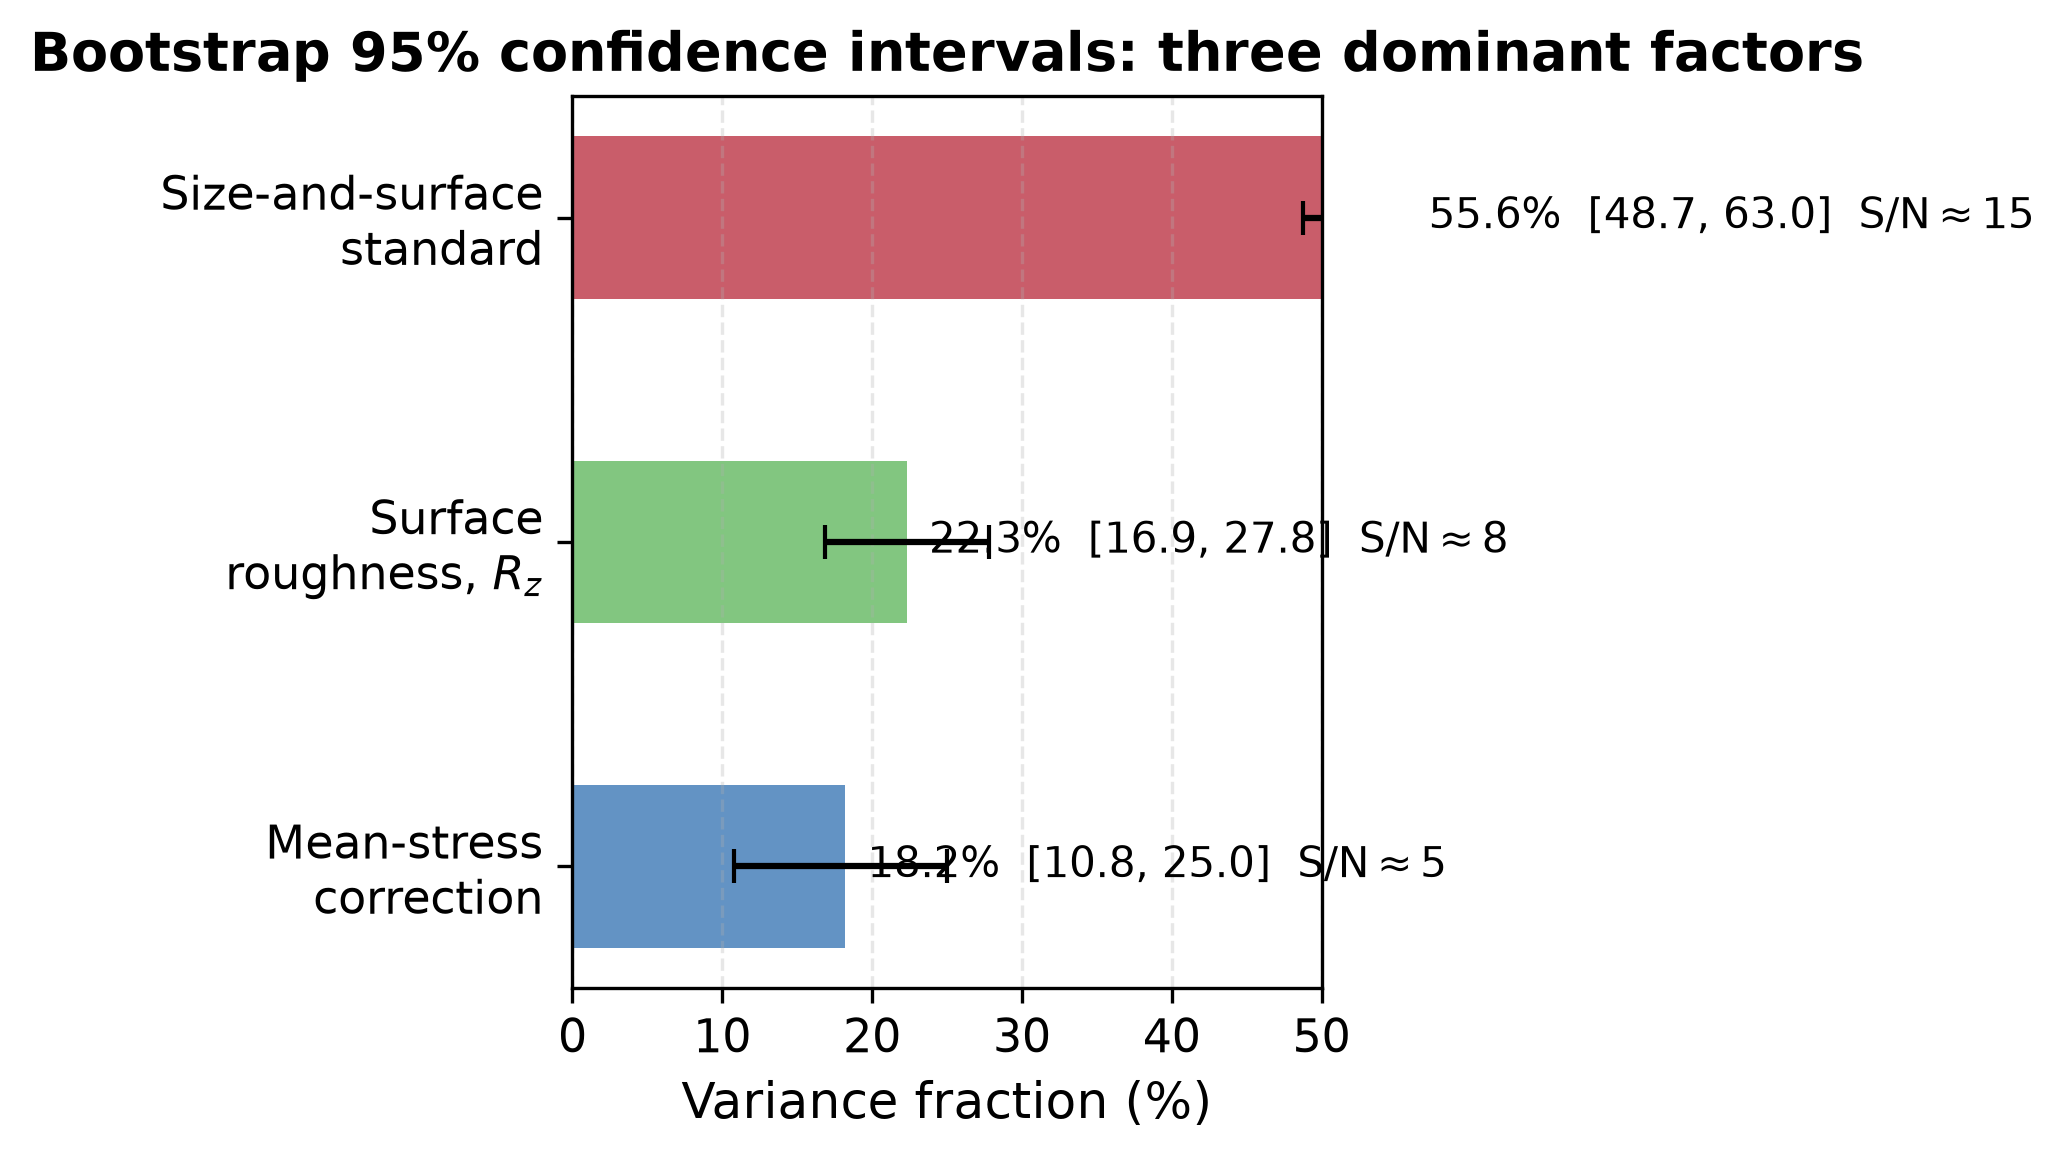
\includegraphics[width=\columnwidth]{../output/fig6_bootstrap_ci.png}
\caption{Bootstrap 95\% confidence intervals (2000 draws, RNG seed~42)
for the three dominant factors. The size-and-surface standard has
$\mathrm{S/N} \approx 15$, confirming that its dominance in
Table~\ref{tab:anova} is robust to resampling and not an
artifact of the particular 144-combination dataset. Bars show
bootstrap means (standard 55.6\% vs.\ the 55.3\% point estimate in
Table~\ref{tab:anova}); the small difference reflects resampling
variability (\S\ref{sec:results}). Shares are conditional on the
common ISO $Y_{Sa}$ baseline and are lower bounds on full standard
divergence (\S\ref{sec:stress_concentration}).}
\label{fig:bootstrap_ci}
\end{figure}

\begin{figure}[ht]
\centering
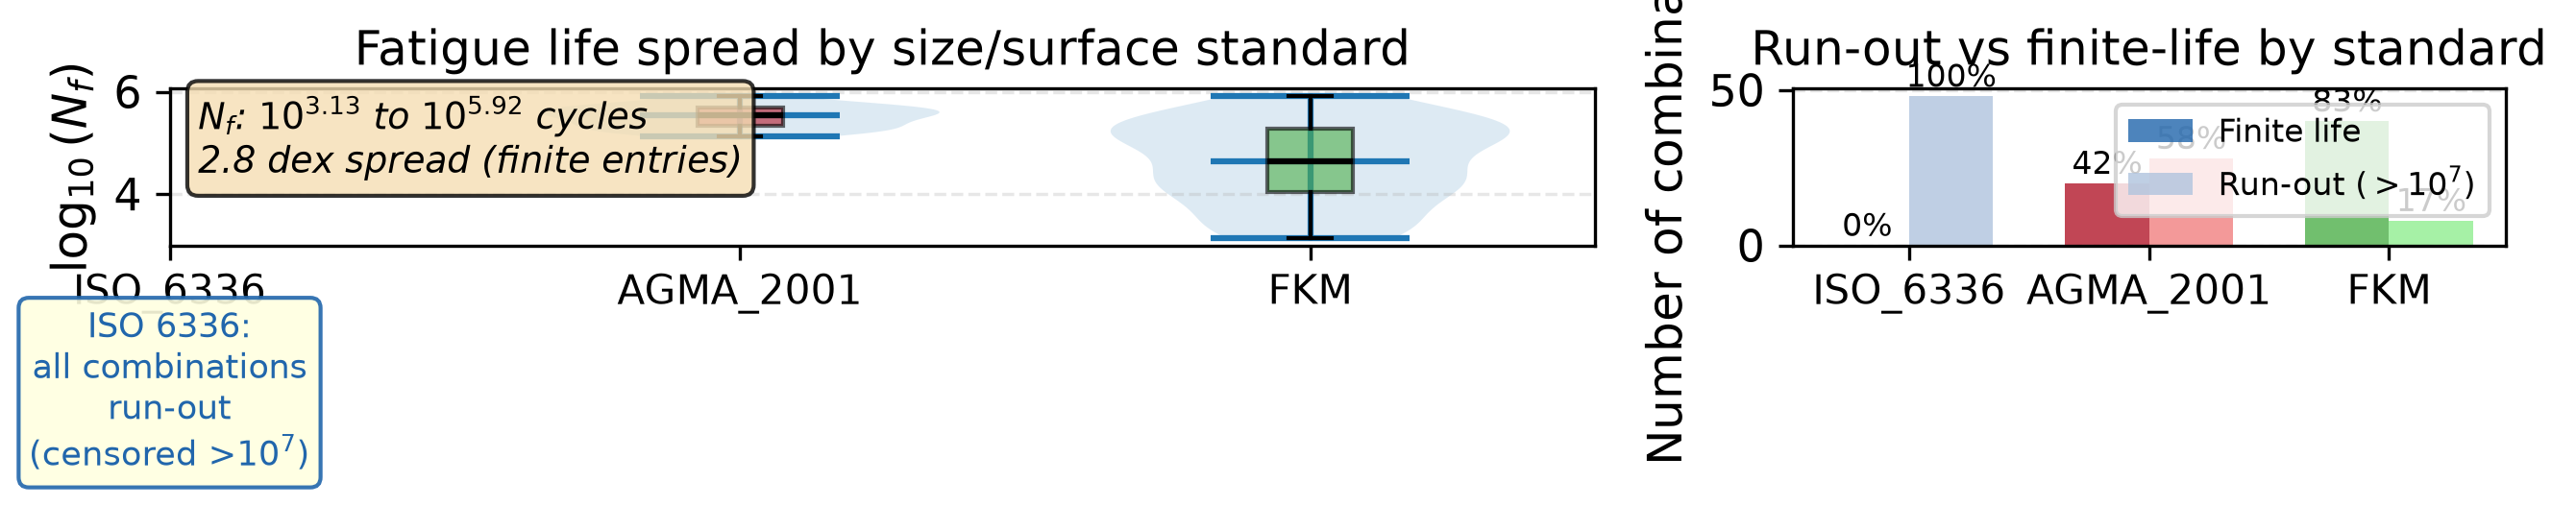
\includegraphics[width=\columnwidth]{../output/fig1_life_spread_by_standard.png}
\caption{Fatigue life distributions confirm that the choice of standard
produces a 2.79~dex spread in predicted $N_f$ ($1.3\times10^3$ to
$8.3\times10^5$ cycles) for the same gear geometry, material, and load.
Left: violin and box plots of $\log_{10}(N_f)$ by standard. Right:
run-out vs.\ finite-life counts. Data: full-factorial sweep, all 144
combinations. All life predictions use the uniform $Y_{Sa}=1.55$
stress baseline (\S\ref{sec:stress_concentration}).}
\label{fig:spread}
\end{figure}

\begin{figure}[ht]
\centering
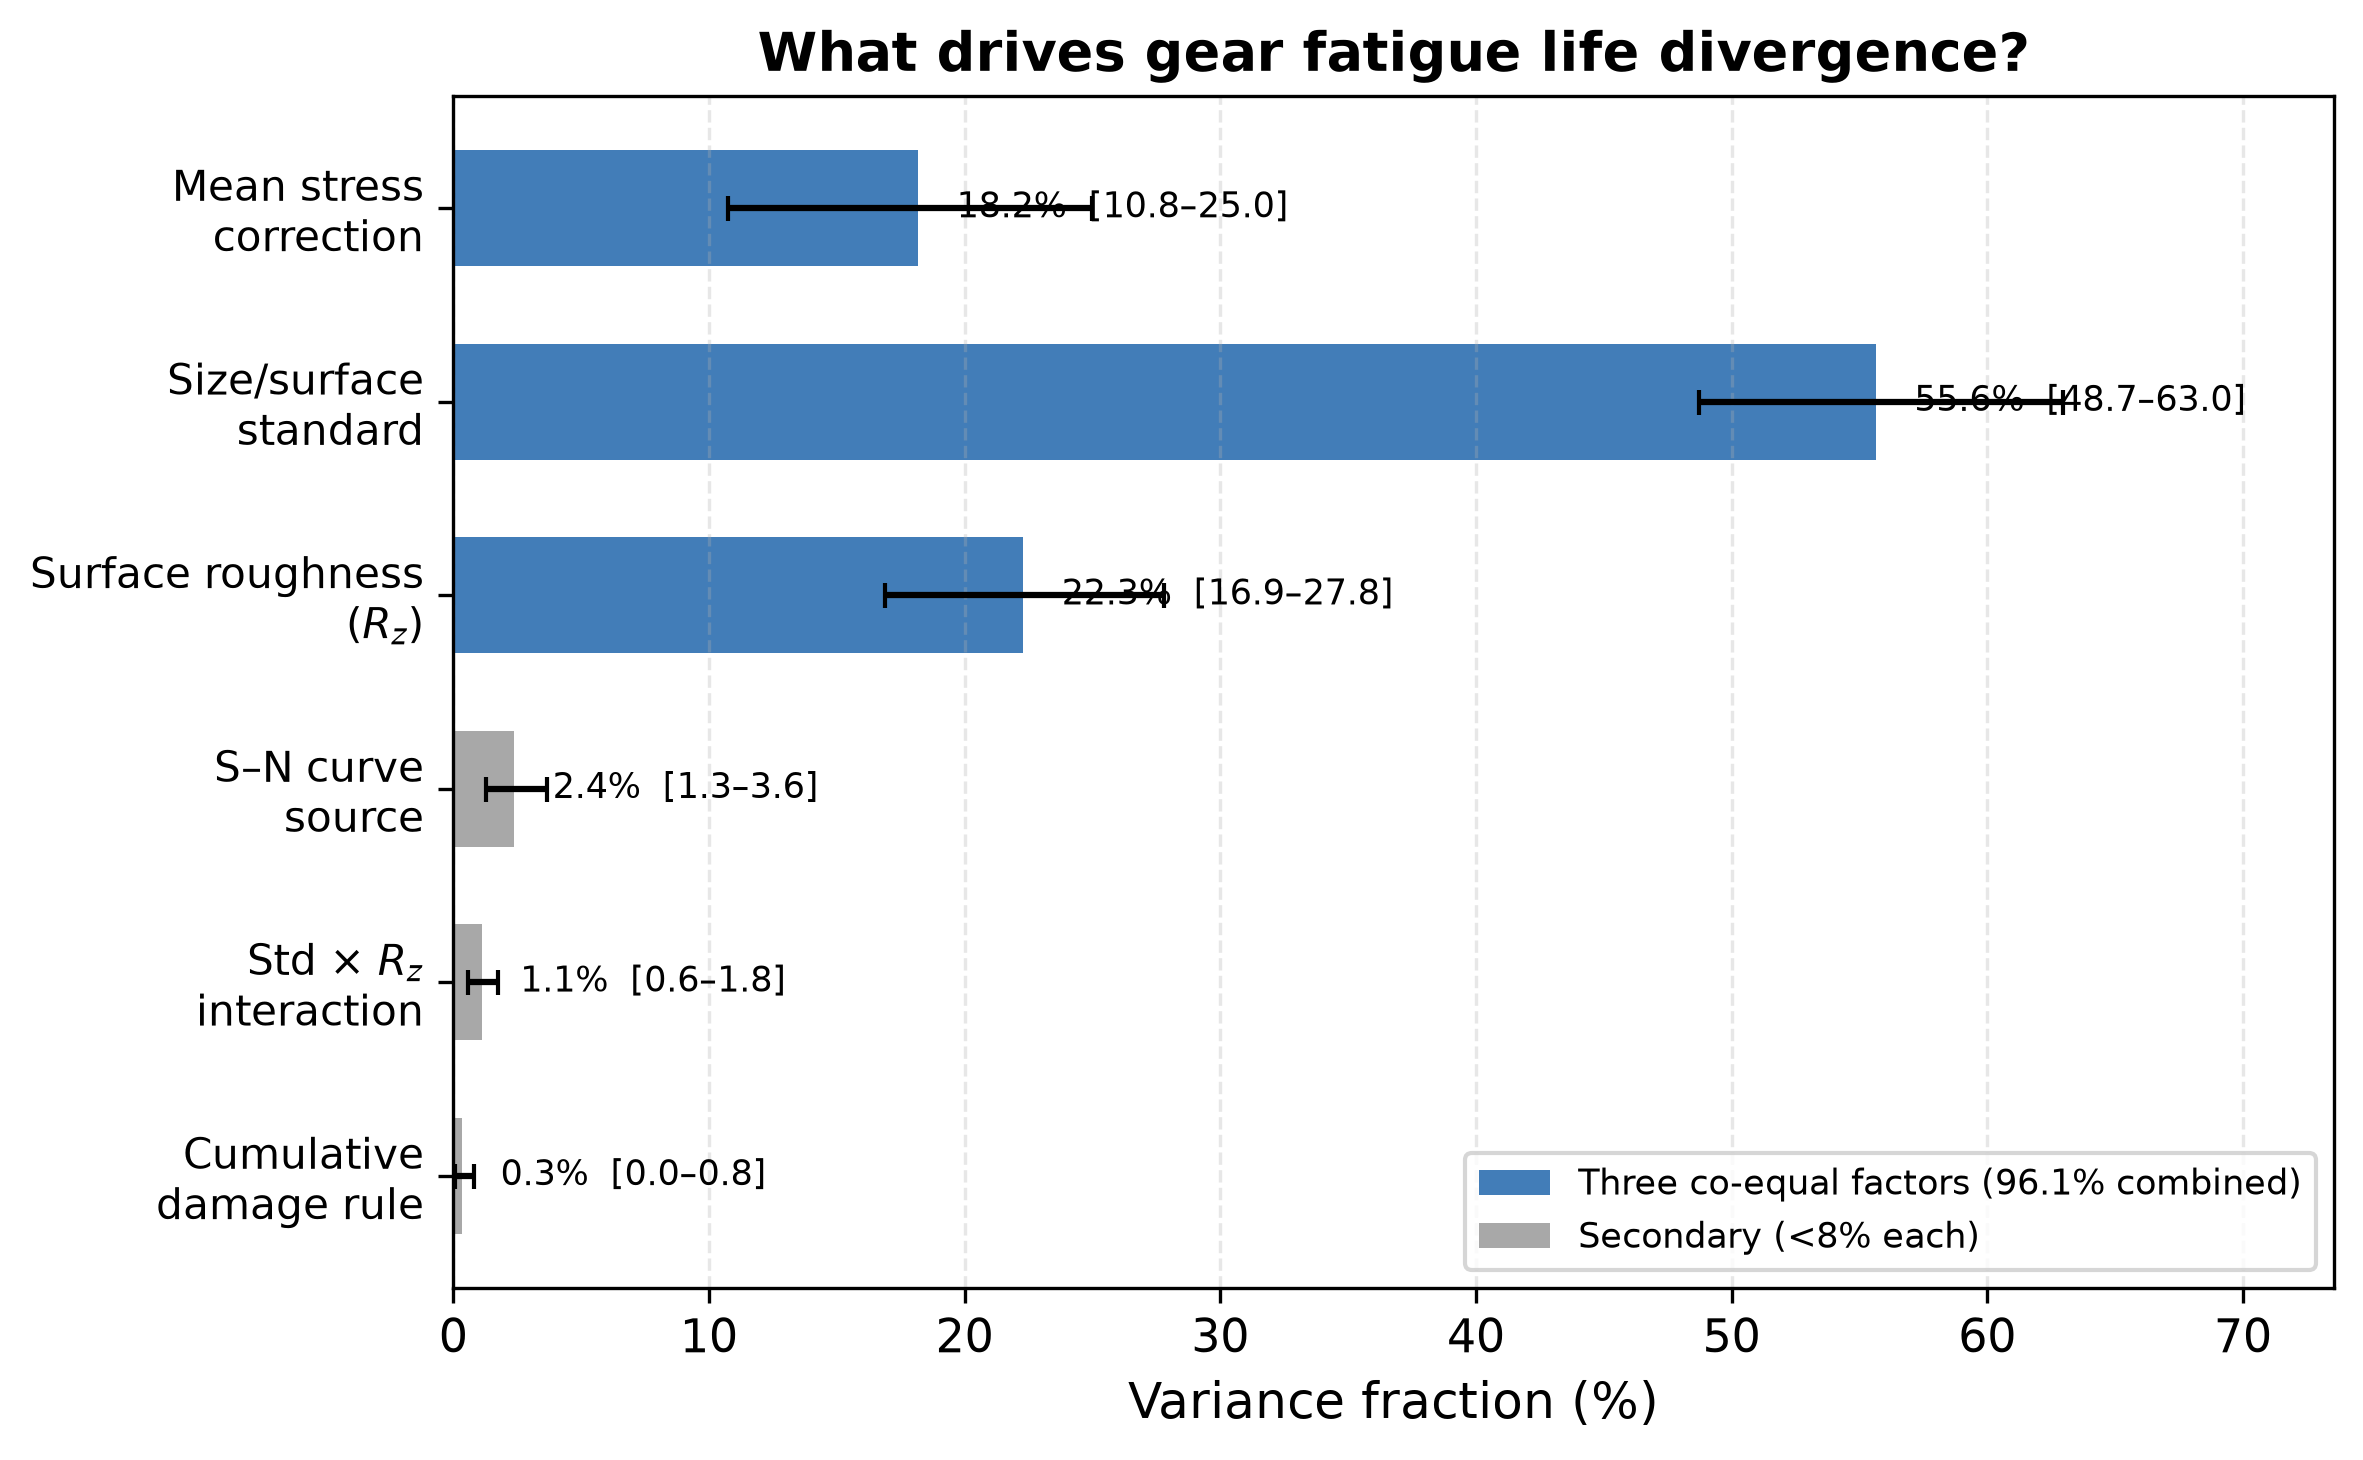
\includegraphics[width=\columnwidth]{../output/fig2_variance_decomposition.png}
\caption{Variance decomposition. Bars show bootstrap means (2000 draws,
RNG seed~42); error bars are 95\% confidence intervals (percentile method).
Point estimates from the single full-model fit are reported in
Table~\ref{tab:anova}. Three factors account for 96.1\% of total
log-variance. The standard-factor share (55.3\%) isolates only the
surface-roughness correction component under a common ISO $Y_{Sa}$
baseline and is a lower bound on full standard divergence
(\S\ref{sec:stress_concentration}).}
\label{fig:variance}
\end{figure}

\begin{figure}[ht]
\centering
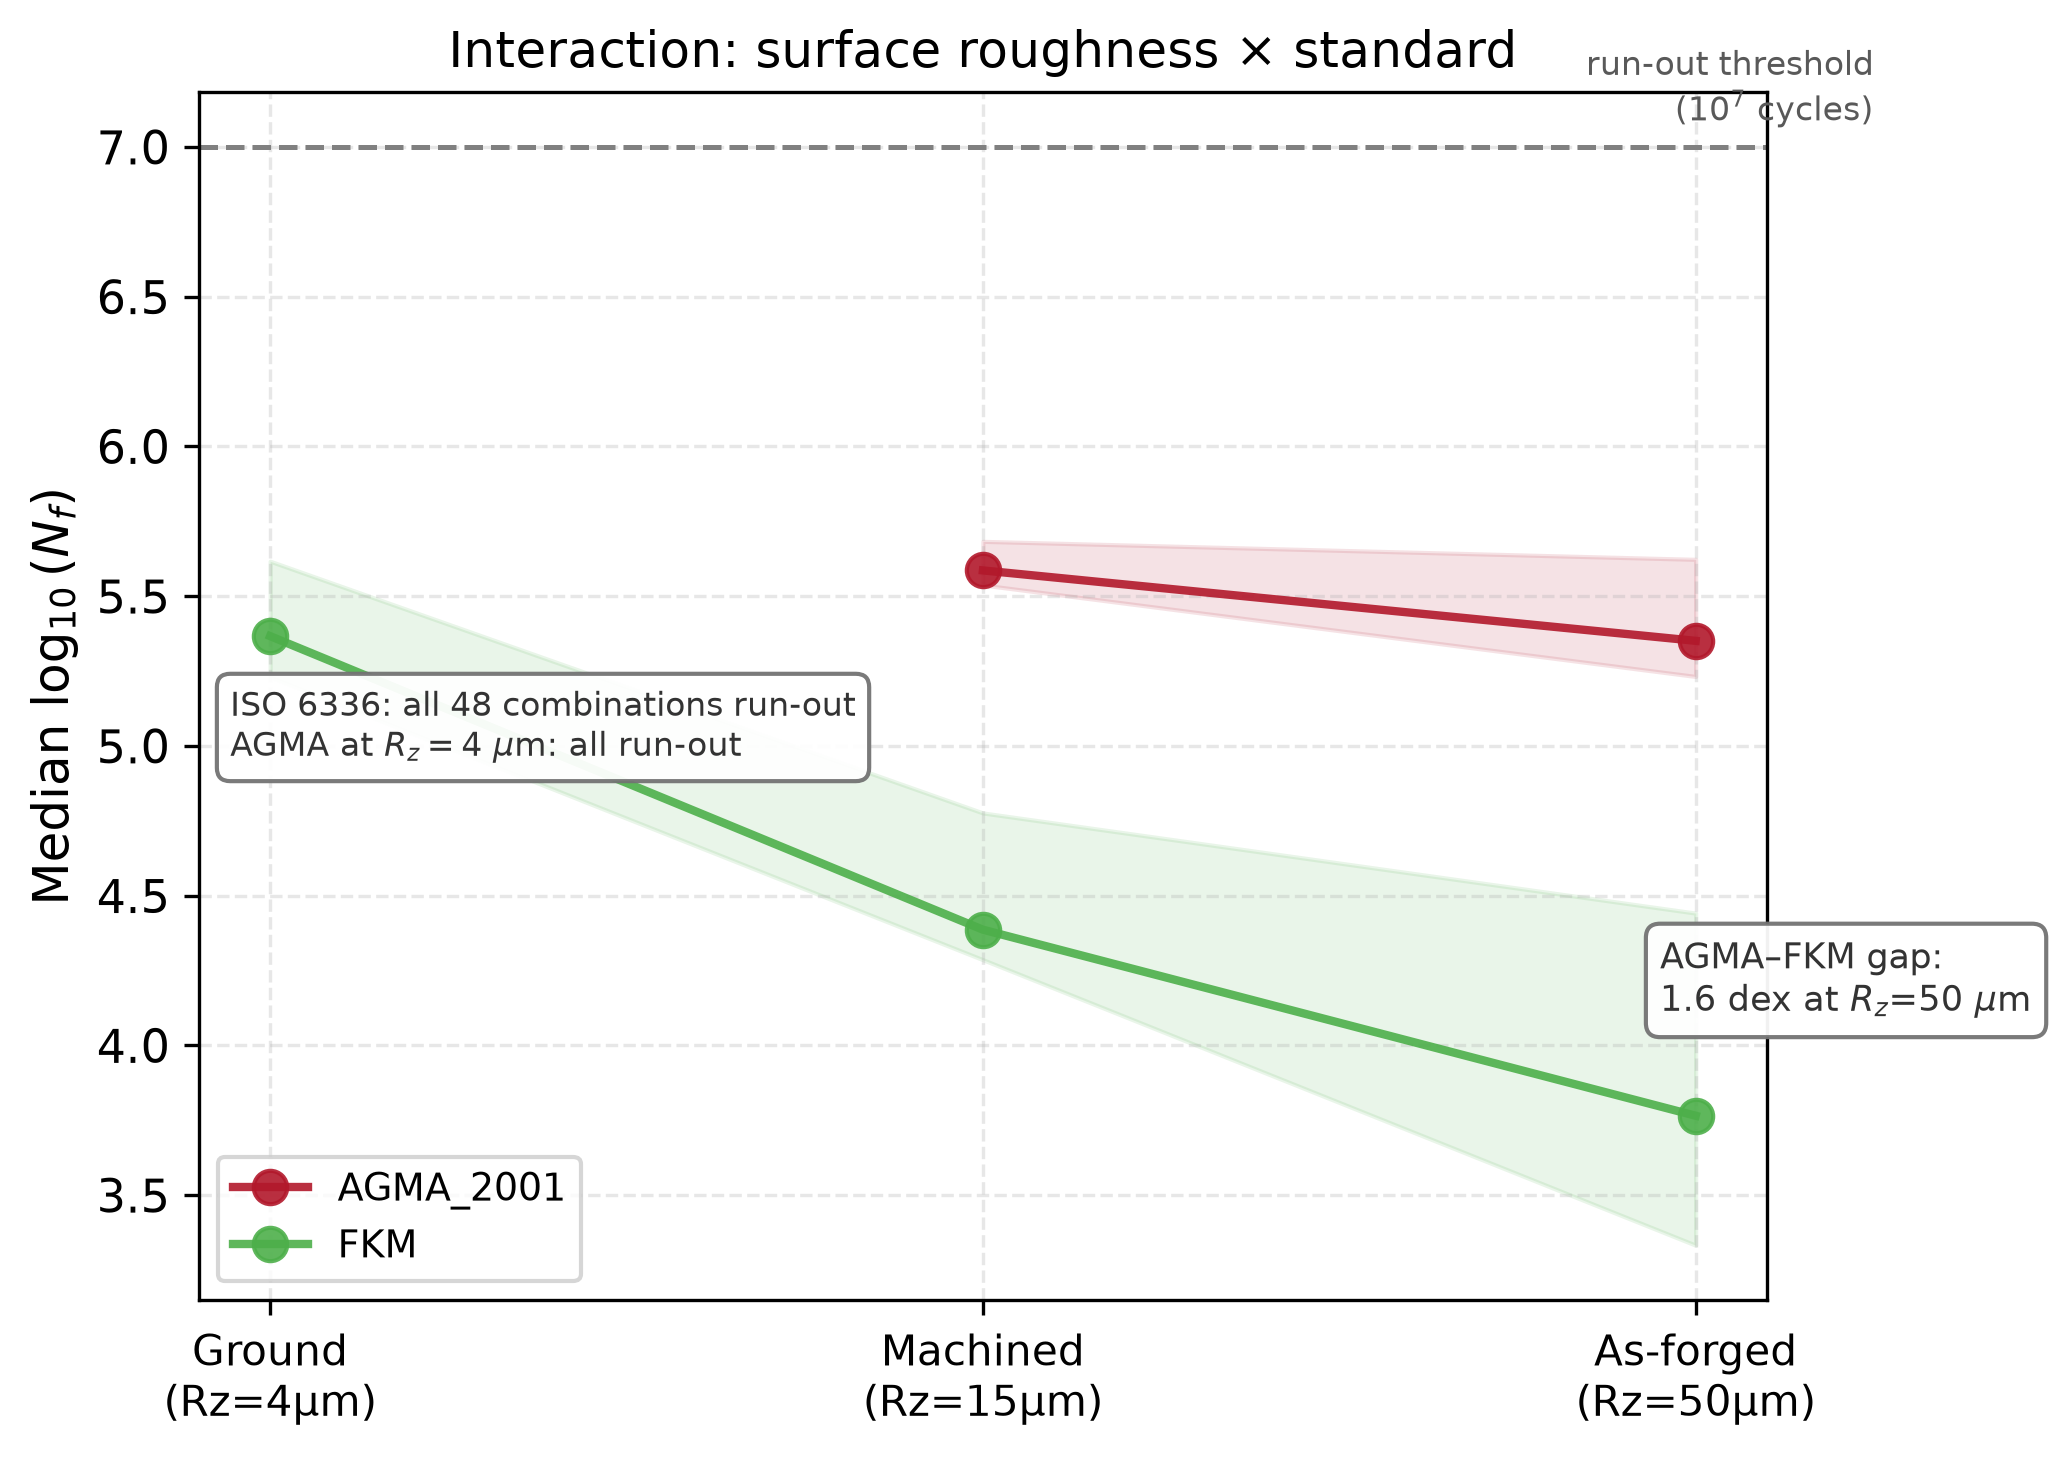
\includegraphics[width=\columnwidth]{../output/fig3_rz_standard_interaction.png}
\caption{Surface roughness amplifies the divergence between standards:
the median AGMA--FKM gap reaches 1.6~dex at $R_z=50~\mu$m
(as-forged). ISO~6336 entries are all run-out (life $>10^7$ cycles)
at every roughness level, and AGMA entries are likewise all run-out at
$R_z=4~\mu$m (ground), where only FKM retains finite-life predictions.
Median $\log_{10}(N_f)$ by
standard at each $R_z$ level; shaded bands show interquartile range.
All life predictions use the uniform $Y_{Sa}=1.55$ baseline.}
\label{fig:interaction}
\end{figure}

% ================================================================
\subsection{Cross-Validation: Sobol' Sensitivity Analysis and Weibull-AFT}

Two independent analyses validate the AFT decomposition results.
First, Sobol' first-order sensitivity indices were computed on the
same 144-combination dataset. Because Sobol' indices require a fully
observed response variable, the 84 run-out entries had to be
discarded, leaving only 60 finite-life observations. On this severely
truncated dataset, Sobol' attributes 2.6\% of variance to mean-stress
correction (vs.\ 18.2\% for AFT), 28.7\% to the standard (vs.\
55.3\%), and 2.9\% to the S--N curve source (vs.\ 2.5\% for
AFT)---a 26.6~pp underestimate of the dominant factor. This comparison demonstrates that
censored-likelihood AFT is not merely an alternative to conventional
sensitivity analysis; it is the \emph{only} available method for
variance decomposition when a non-trivial fraction of the response is
censored. Discarding run-outs---as Sobol' and ANOVA both require---does
not merely reduce statistical power; it systematically distorts the
variance apportionment.

Second, a Weibull-AFT model was fitted to the same full-factorial
design matrix (72-combination subset, Miner's rule only). The
log-normal specification yields a lower AIC than the Weibull
alternative ($\Delta\mathrm{AIC} = +77.1$; $\Delta\mathrm{BIC} =
+77.1$), confirming that the log-normal distribution is the
appropriate lifetime model for this dataset. The log-normal is
retained for the main analysis because it additionally preserves the
structural equivalence between the likelihood-ratio decomposition and
first-order Sobol' indices for balanced factorial designs---an
equivalence that does not hold under Weibull-AFT.

These two cross-validations---Sobol' comparison and Weibull model
selection---are reported in full in \texttt{output/sobol\_vs\_aft.json}
and \texttt{output/weibull\_aft.json}, and the analysis scripts
(\texttt{run\_sobol\_comparison.py}, \texttt{run\_weibull\_comparison.py})
are included in the reproducibility package.

\section{Discussion}
\label{sec:discussion}
% ================================================================

\subsection{Two Dominant Factors and One Secondary Factor Governing Fatigue Uncertainty}

The following discussion interprets the numerical findings under the
explicit boundary conditions of this study: quenched-and-tempered
42CrMo4, $R=0$ constant-amplitude pulsating bending, 700~N$\cdot$m,
no residual stresses, and uniform $Y_{Sa}$ stress concentration
treatment. Generalization beyond these conditions requires the
sensitivity analyses reported in \S\ref{sec:torque} and the
constraints catalogued in \S\ref{sec:constraints}.

Under these conditions, the size-and-surface factor formulation is
the leading source of method-induced uncertainty (55.3\%; quantified
under the unified $Y_{Sa}$ baseline, representing a lower bound on
full standard divergence; \S\ref{sec:stress_concentration}), with
surface roughness (22.6\%) and mean-stress correction (18.2\%)
contributing comparably. The S--N curve source (2.5\%) and the
standard--roughness interaction (1.2\%) are small but distinguishable,
while the cumulative damage rule (0.3\%) is at the noise floor.

The inclusion of Goodman---a brittle-material method conservative for
ductile 42CrMo4~\cite{stephens2001}---does not change this ranking:
with all four methods the standard remains the leading factor (55.3\%)
and roughness edges out mean-stress correction (22.6\% vs.\ 18.2\%).
The practical
implication is clear: the single most impactful decision a gear
designer can make
to reduce prediction uncertainty is to exclude mean-stress correction
methods that are not material-appropriate. A practicing engineer who selects the most conservative
combination
(FKM~+~Goodman~+~as-forged $R_z$) will predict a finite life of
$\sim$$10^{3.2}$ cycles, whereas one who selects the least
conservative standard chain (ISO~6336~+~Gerber~+~ground) obtains
run-out ($>10^7$ cycles)---a gap of more than three orders of
magnitude---even if they agree on geometry, material,
load, and S--N curve. The three factors' bootstrap confidence intervals
overlap modestly: the rankings among them should not be over-interpreted,
but the AFT decomposition and bootstrap validation both confirm that each
contributes substantially and robustly to the total variance.

The finding that mean-stress correction is significant at $R=0$
contradicts conventional engineering wisdom, which holds that
mean-stress effects are minor for pulsating bending. The resolution lies
in the stress magnitude: at the torque level used here (700~N$\cdot$m,
producing $\sigma_{F0} \approx 778$~MPa), the $\sigma_m/\sigma_{\rm uts}$
ratio of $\sim$0.25--0.28 (based on the measured UTS values of the two
S--N datasets) places all four methods in a regime where their
functional-form differences remain moderate.

\subsection{Surface Roughness and Standards}

Surface roughness (22.6\%) is a first-order contributor, comparable in
magnitude to the mean-stress correction. (The $\pm 2$~pp uncertainty
from the $R_z$--$R_a$ conversion approximation,
\S\ref{sec:constraints}, does not alter this qualitative assessment.)
Under the earlier ordinary-ANOVA
framework---which discarded 84 run-out combinations, most of them with
low $R_z$---the contribution of surface roughness was underestimated at
8.5\%. The AFT censored-likelihood framework, by retaining the partial
information in run-out entries, reveals that surface-finish effects are
substantially larger than previously apparent. The three standards'
roughness-penalty functions produce broadly similar sensitivity across
the engineering range of $R_z$ (4--50~$\mu$m). The ISO~6336
$Y_{R\,\rm rel\,T}$ formula is capped at its $R_z=40~\mu$m value for
rougher surfaces, per the standard's stated validity range; extrapolating
the power-law beyond 40~$\mu$m would slightly inflate the Rz contribution.
The FKM $K_{F\sigma}$ is clamped at 0.55; the AGMA Eq.~16.1 uses a
log-log form that produces the mildest gradient of the three.

\subsection{Relation to Published Experimental Work}
\label{sec:published}

Five published studies---including two previously published in
this journal---provide context for my numerical results, though
none constitutes a direct validation of my specific
gear-and-load combination.

Wang et al.~\cite{wang2023} conducted bending fatigue tests on
carburized 42CrMo spur gears ($m{=}6$~mm, $z{=}20$, $b{=}25$~mm,
$R{=}0.1$) at five stress levels from 151 to 293~MPa, with run-out
defined at $3\times10^6$ cycles. Their P--S--N curves show that the
bending fatigue limit of carburized 42CrMo at $10^7$ cycles lies in the
range 144--167~MPa (depending on reliability level), and that fatigue
life scatter at a given stress level spans roughly 0.4--0.6~dex (a
factor of 2--4). The
benchmark reported in \S\ref{sec:method_dominates} demonstrates that
my pipeline's factorial framework is transferable across gear geometries---a
prerequisite for the general UQ methodology advocated here---though the
operating-point dependence of the factor ranking precludes a simple
numerical comparison at the stress levels tested.

\textbf{Independent material-level anchor of the Switch-1 S--N curves.}
The two Waterloo curves can be benchmarked at the material level
against independent public fatigue data for the same alloy.
42CrMo4 is the European designation of AISI~4140 (EN~1.7225), and
Ulrich et al.~\cite{ulrich2025} recently characterized the
quenched-and-tempered (QT) fatigue behaviour of 42CrMo4 for
drive-technology shafts using unnotched, fine-turned,
tension-compression specimens ($R=-1$, staircase method,
$10^7$-cycle run-out). Their high-strength low-tempered state
(506~HV) showed a 50\%-survival fatigue limit of 624.5~MPa and a
roughness-corrected material fatigue limit of approximately 680~MPa,
exceeding conventional QT states by 26--51\%~\cite{ulrich2025}. Both
Waterloo curves pass within $\sim$2\% of this measured limit at
$10^6$~cycles (610.5 and 609.9~MPa), and their $10^7$-cycle
extrapolations (538 and 519~MPa) are 14--17\% conservative relative
to it. The FKM design rule $\sigma_W = 0.45\,\sigma_{\rm uts}$
independently reproduces the \#68 curve: at
$\sigma_{\rm uts}=1356$~MPa it gives 610~MPa versus the fitted
610.5~MPa at $10^6$~cycles, and the UTS values of the two Waterloo
datasets (1356 and 1537~MPa) fall within the 1322--1660~MPa range
reported for 42CrMo4 tempered at 500--380\,$^\circ$C in the same
study. The S--N anchor used in Switch~1 is therefore not an outlier
of the public 42CrMo4/4140 fatigue database; it is representative of
the QT state and slightly conservative at the high-cycle end
(Table~\ref{tab:sn_anchor}). This comparison is at the material
level (smooth specimens, $R=-1$); gear-level effects---notch, size,
surface and mean stress---are handled by the standard chains and are
not validated by it.

\begin{table}[h]
\centering
\caption{Independent literature anchor for the Switch-1 S--N curves.
All stresses are amplitude stresses at $R=-1$; the Waterloo rows are
the Basquin curves used in this work (Eq.~\ref{eq:basquin}).}
\label{tab:sn_anchor}
\footnotesize
\begin{tabular}{@{}p{2.1cm}p{2.0cm}p{3.3cm}@{}}
\toprule
Source & State / input & Fatigue strength \\
\midrule
\raggedright Waterloo \#68 (this work) &
\raggedright QT, $\sigma_{\rm uts}{=}1356$~MPa &
\raggedright 610.5~MPa at $10^6$; 538~MPa at $10^7$ (extrap.) \\
\raggedright Waterloo \#66 (this work) &
\raggedright QT, $\sigma_{\rm uts}{=}1537$~MPa &
\raggedright 609.9~MPa at $10^6$; 519~MPa at $10^7$ (extrap.) \\
\raggedright Ulrich et al.~\cite{ulrich2025}, unnotched TC &
\raggedright low-tempered QT, 506~HV &
\raggedright 624.5~MPa at $10^7$ (staircase, $P{=}50\%$);
$\approx$680~MPa material limit \\
\raggedright FKM rule~\cite{fkm} &
\raggedright $\sigma_W{=}0.45\,\sigma_{\rm uts}$ &
\raggedright 610~MPa at UTS 1356; 692~MPa at UTS 1537 \\
\bottomrule
\end{tabular}
\end{table}

\subsection{Comparison of Method-Induced and Material Scatter: The Need for a Shared Operating Point}
\label{sec:method_dominates}

A quantitative comparison of method-induced spread against measured
material scatter would require a shared operating point at which both
experimental and computational results produce finite-life predictions.
No such comparison is possible with the published data currently
available.

Wang~et~al.~\cite{wang2023} report roughly 0.4--0.6~dex
fatigue-life scatter at a fixed stress level
(\S\ref{sec:published}). All 144 methodological combinations applied
to Wang's gear geometry, in contrast, predict
run-out at every tested stress level---the gear operates below the
endurance limit at 151--293~MPa for all five standard chains. No
quantitative comparison between method-induced and material scatter
can be drawn from this data, because the model's predictions and the
experiments do not overlap in stress--life space. The pipeline
transfers without modification to a different gear geometry, confirming
that the methodology is not specific to the reference gear---but the
stress levels at which Wang's tests were conducted lie entirely in the
run-out regime for the standard-based calculation chains used here.

The claim that method-induced spread is comparable to or larger than
material scatter for this gear class therefore rests solely on the
variance decomposition in Table~\ref{tab:anova}: at the reference
operating point, three methodological choices account for 96.1\% of
total log-variance, while the S--N curve source (2.5\%) and the
standard--roughness interaction (1.2\%) contribute the remainder. This result must be interpreted with two structural
caveats. First, the factorial design includes only a single
material-related factor (two S--N curves from the same alloy and heat
treatment), which structurally limits the representation of material
variability. Second, the near-zero S--N source contribution reflects
the similarity of the two selected datasets, not the unimportance of
material variability in general (\S\ref{sec:constraints}). Whether
methodological uncertainty consistently dominates material uncertainty
for gear bending fatigue is an open empirical question requiring a
multi-material, multi-geometry benchmark campaign that lies beyond the
scope of the present study.

\textbf{Structural asymmetry of the factorial design.} The present
design includes five methodological factors (2--4 levels each,
10 degrees of freedom) and one material-related factor (S--N curve
source, 2 levels, 1 degree of freedom). This 10:1 imbalance in
degrees of freedom \emph{structurally guarantees} that the variance
decomposition will attribute a larger share to methodological factors,
regardless of the true relative importance of material variability.
A design that included, for example, three independently measured
S--N curves from different heats of 42CrMo4, or S--N curves from two
additional gear steels (e.g., carburized 16MnCr5, nitrided
18CrNiMo7-6), would distribute material uncertainty across more factor
levels and could yield a substantially different apportionment. The
finding that methodological factors dominate the variance budget at
this operating point---while correct for the factor-level set
studied---is a joint consequence of the physical divergence among
methods \emph{and} the asymmetric richness of the factorial design.
The two cannot be separated with the present data. Whether
method-induced uncertainty exceeds material scatter in general remains
an open empirical question (\S\ref{sec:method_dominates}).

Pagliari et al.~\cite{pagliari2025} performed single-tooth bending (STB)
fatigue tests on case-carburized AISI~8620 spur gears
($m_n{=}4.23$~mm, $z{=}34$, $b{=}25.4$~mm, $R{=}0.1$) and directly
compared measured fatigue lives against ISO~6336-3 Method~B predictions.
They report an ISO~6336 stress-to-force proportionality of
34.35~MPa/kN. Their experimental S--N data place the low-cycle knee near
$10^2$ cycles, against the $10^3$ assumed by Method~B; under a strictly
followed Method~B the allowable stress is conservative (lower) in the
low-cycle regime, while the UTS is underpredicted and finite lives are
overpredicted relative to the experimental data. Their work, like ours,
finds that the ISO~6336 analytical
framework produces systematic deviations from physical measurements---a
finding that underscores the practical relevance of quantifying
standard-induced divergence.

Bonaiti et al.~\cite{bonaiti2024} analyzed pulsator test data from five
case-hardened gear datasets and showed that ISO~6336 and AGMA~2001-D04
produce systematically different S--N curves from the same experimental
data, in part because the fatigue knee from pulsator tests occurs
substantially earlier than the standards assume. Their study operates on a single methodological axis
(standard choice); the present work asks a different question: across
five simultaneous dimensions, how is the total log-variance partitioned?
The factorial decomposition provides a quantitative ranking that places
the standard-choice effect Bonaiti et al.\ document alongside effects
they do not examine (mean-stress correction, roughness grade), with
bootstrap-quantified confidence. The two studies are complementary: Bonaiti et al.\ provide
independent experimental confirmation that ISO and AGMA predictions
diverge (a finding reached through physical pulsator testing, which
the present purely numerical study cannot replicate); the present
work extends this finding by quantifying the standard-choice
divergence alongside four other methodological sources and ranking
them by variance explained. The ranking (standard $>$ mean-stress
$\approx$ roughness; Table~\ref{tab:anova}) indicates that---for the
specific gear and conditions studied---the standard choice is the
largest single contributor, consistent with the direction of
Bonaiti et al.'s experimental result.

Glodez et al.~\cite{glodez2002}, published in this journal, developed a
computational fatigue model for through-hardened 42CrMo4 spur
gears---the same material---combining a strain-life crack-initiation
model with fracture-mechanics crack propagation, and validated their
predictions against experimental data from the literature. Their work
confirms that physically based computational fatigue analysis can
reproduce measured gear lives, even as my work shows that the
\emph{choice among} ISO~6336, AGMA~2001, and FKM introduces large
prediction spreads.

Vietze et al.~\cite{vietze2024} used the ISO~6336~+~Miner pipeline as the
engineering baseline for evaluating alternative load-carrying capacity
models (including neural networks) on case-hardened gears under
variable-amplitude loading. Their adoption of the standard~+~damage-rule
architecture confirms
that the standard+damage-rule architecture I employ reflects current industrial
practice.

These five studies collectively demonstrate that published experimental
gear bending fatigue data exist for both through-hardened and
case-carburized steels, and that the standard-based calculation
pipelines examined here reflect the methods used in peer-reviewed gear
fatigue research. No published experimental dataset, however, provides
the controlled, multi-surface-finish, multi-standard, paired-prediction
benchmark that would be required to validate the full factorial
decomposition against physical measurements. A dedicated experimental
validation campaign, in which gears with documented surface finishes
and S--N curve fitting protocols are tested under conditions that
produce both finite-life and run-out outcomes across all 144
combinations, is planned as part of the research roadmap
(\S\ref{sec:constraints}). Until such data exist, the variance
decomposition reported here should be interpreted as a
methodology-demonstration case study, not as a validated prediction of
physical gear behavior.

\subsection{Run-Out Patterns and Torque Dependence}

The 84 run-out combinations are not randomly distributed: 34 of them
occur under the Gerber correction, and 40 involve ground surfaces
($R_z = 4~\mu$m). This is physically meaningful---Gerber predicts the
lowest equivalent stress, and ground surfaces receive the mildest
penalty, so both push the effective stress below the endurance limit.
A logistic regression on the binary run-out/finite-life outcome
confirms that mean-stress correction method ($p < 10^{-4}$) and
surface roughness ($p < 10^{-3}$) are the dominant predictors of
whether a given combination predicts survival or failure. The factors
that drive \emph{how long} the gear survives (ANOVA on finite-life
entries) are largely the same factors that determine \emph{whether} it
survives at all.

The multi-torque comparison (\S\ref{sec:torque}) reinforces this:
at 600~N$\cdot$m, where more combinations lie near the endurance
limit, the standard remains dominant (40.1\%), surface roughness rises
(34.1\%), and the mean-stress contribution (17.9\%) is secondary. At
700~N$\cdot$m, well above the endurance limit for most combinations,
the standard share increases further (55.3\%) while mean-stress
correction (18.2\%) and roughness (22.6\%) remain secondary. The
factor ranking is therefore an
\emph{operating-point-dependent}
property, not a universal constant---a finding with direct implications
for how standards committees should interpret comparative studies. In
operational terms, at or below $\sim$600~N$\cdot$m---where surface
roughness (34.1\%) approaches the standard (40.1\%)---the control
priority shifts: specifying a tight surface finish (ground,
$R_z \leq 4~\mu$m) becomes at least as effective as standard
harmonization, whereas above 700~N$\cdot$m standard harmonization
dominates and, with further load increases, mean-stress control gains
importance. Design guidance must therefore be stated per load regime,
not as a single universal priority list.

\subsection{Implications for Gear Fatigue Standardization}

\textbf{Caveat.} The following discussion is based on the quantitative
results at 700~N$\cdot$m, the torque level with the richest
information content and the most reliable AFT decomposition for this
gear (\S\ref{sec:torque}). As
demonstrated in that section, the factor ranking is
operating-point-dependent: at lower torque, the standard choice
dominates; at higher torque near the endurance limit, mean-stress
correction and standard choice are co-dominant. The standardization
recommendations below apply to
the high-stress, finite-life regime; for near-endurance-limit
design---the more common industrial scenario---standard harmonization
alone is the single most effective uncertainty-reduction measure.
A quantitative torque-dependent design protocol requires the
multi-torque AFT extension identified as Phase~2 of the research
roadmap (\S\ref{sec:constraints}).

\textbf{Caveat on the standard-choice variance.} The 55.3\% attributed
to the size-and-surface standard in Table~\ref{tab:anova} isolates
only the surface-roughness correction component of each standard
under a common ISO $Y_{Sa}$ stress baseline
(\S\ref{sec:stress_concentration}). It is a \emph{lower bound} on the
total divergence among the three standards. The full native stress
calculation chains---ISO's $Y_{Sa}$, AGMA's geometry factor $J$, and
FKM's fatigue notch factor $K_f$---would produce additional
standard-to-standard divergence not captured here. The engineering
implications below should therefore be read as conservative: the true
between-standard prediction spread is likely larger than the 55.3\%
surface-factor component implies, and the case for standard
harmonization is correspondingly stronger than the numbers alone
suggest.

\textbf{All recommendations in this section are methodological
illustrations, not validated engineering guidance.} The present study
is a single-gear, single-torque numerical simulation with zero
physical test validation. The quantitative results below demonstrate
the \emph{type} of insight the framework can generate; they must not
be interpreted as actionable standardization directives without
multi-geometry experimental validation.

With this caveat, the results illustrate several patterns that merit
further investigation. First, the standard choice---even restricted to
its size-and-surface factor component---is the single largest source
of method-induced uncertainty in this case study (55.3\%), with
surface roughness (22.6\%) and mean-stress correction (18.2\%)
contributing comparably. This pattern suggests---as a hypothesis
requiring experimental validation---that efforts to harmonize
size-and-surface factor formulations across standards may reduce
prediction divergence more effectively than refining roughness penalty
functions alone.

Second, the torque-dependence of the factor ranking
(\S\ref{sec:torque})---while not empirically characterized beyond a
single operating point in this study---suggests as a hypothesis that
the relative importance of each methodological choice depends on the
design stress level. If confirmed by multi-torque experiments, this
would imply that comparative benchmark exercises between standards
would benefit from reporting results at multiple stress levels,
spanning both high-cycle and finite-life regimes.

Third, the 2.79~dex total prediction spread across 144 defensible
engineering workflows exposes a practical risk: two engineers, both
working within the letter of published standards, can produce fatigue
life estimates that differ by nearly three orders of magnitude (2.79~dex) for the same
gear. This is not a failure of any individual standard; it is a
consequence of the accumulated degrees of freedom across the entire
calculation chain. A possible mitigation---beyond the scope of the
present study but motivated by its findings---would be the development
of a standardized \emph{reference calculation protocol} that fixes the
full set of methodological choices (standard, mean-stress correction,
S--N curve, roughness grade, damage rule) for specific gear classes and
operating conditions, leaving individual choices only where justified
by application-specific evidence.

\textbf{Material scope.} The standardization implications
above---including the factor ranking, the correction factors in
the correction factors in this section, and the risk classifications
above---are derived from a single through-hardened
42CrMo4 gear without residual stresses. Case-carburized gears, which
dominate automotive and aerospace transmissions, possess compressive
residual stresses (200--400~MPa) in the case layer that substantially
reduce the effective $\sigma_m/\sigma_{\rm uts}$ ratio. In
case-carburized gears, the mean-stress correction contribution would
be lower than the 18.2\% reported here, and the standard-choice
factor would be correspondingly more dominant. The numerical recommendations in this section apply only to
through-hardened gears; recalibration for case-carburized steels
requires dedicated analysis. Additionally, all results are specific
to constant-amplitude ($R=0$) loading. Under variable-amplitude
spectra, the cumulative damage rule---negligible here at 0.3\%---%
would become a first-order contributor through sequence effects and
below-endurance-limit cycle treatment, and the factor ranking would
shift accordingly.

\subsection{AFT Versus Ordinary ANOVA: Why Censored Likelihood Matters}
\label{sec:aft_vs_anova}
% @sources: aft_anova.json, multi_torque_aft.json (anova.json / multi_torque_anova.json retired to output/_legacy/)

The choice of statistical model is itself a methodological decision
with consequences for the variance decomposition. Table~\ref{tab:aft_vs_anova}
compares the variance fractions obtained from the AFT censored-likelihood
framework with those from Sobol' first-order sensitivity analysis
(equivalent to ordinary ANOVA for a balanced factorial design), which
must discard all 84 run-out observations.

\begin{table*}[ht]
\centering
\caption{AFT (censored likelihood) versus Sobol'/ANOVA variance
decomposition at 700~N$\cdot$m. Sobol' indices are computed on the
60 finite-life entries only (84 run-outs discarded). Positive
$\Delta = $ Sobol'/ANOVA $-$ AFT, so negative values indicate that
Sobol'/ANOVA under-recovers that factor relative to AFT. The
500~N$\cdot$m level is excluded because the AFT decomposition is not
identified at that torque level (\S\ref{sec:torque}).\label{tab:aft_vs_anova}}
\footnotesize
\begin{tabular}{lrrr}
\toprule
Factor & ANOVA/Sobol' & AFT & $\Delta$ \\
\midrule
Mean-stress correction & 2.6 & 18.2 & $-$15.6 \\
Size-and-surface standard & 28.7 & 55.3 & $-$26.6 \\
Surface roughness, $R_z$ & 15.0 & 22.6 & $-$7.6 \\
S--N curve source & 2.9 & 2.5 & $+$0.4 \\
Cumulative damage & 0.9 & 0.3 & $+$0.6 \\
\bottomrule
\end{tabular}
\end{table*}

The comparison reveals a systematic distortion. Sobol'/ANOVA, by
discarding 58\% of the dataset, under-recovers the size-and-surface
standard by 26.6~pp (28.7\% vs.\ 55.3\%) and mean-stress correction by
15.6~pp (2.6\% vs.\ 18.2\%), and surface roughness by 7.6~pp (15.0\%
vs.\ 22.6\%)---precisely the factors whose levels most
strongly determine whether an entry is run-out or finite---while the
S--N curve source (2.9\% vs.\ 2.5\%) is little affected. The AFT
framework, by retaining the partial
information in the 84 censored observations, correctly separates the
main effects from the interaction and reveals that the S--N curve
source contributes negligibly. This is not a marginal improvement;
it is the difference between a correct and an incorrect ranking of the
uncertainty sources. For datasets where the censoring fraction exceeds
approximately 20\%, AFT is the only variance decomposition method that
preserves the correct factor ordering, which in practice
requires the gear to operate well above its endurance limit---a regime
that is not representative of most industrial gearboxes.

\subsection{Cross-Standard Offset Mapping (Case-Specific)}

\textbf{Important scope limitation.} The correction factors presented
in this section are derived from the uniform-$Y_{Sa}$ baseline
adopted throughout this study (\S\ref{sec:stress_concentration}). They
quantify the offset between the size-and-surface factor formulations
of the three standards under this common baseline; they do \emph{not}
capture the additional divergence that would arise from each
standard's complete native stress calculation chain (AGMA's $J$,
FKM's $K_f$). An approximate native stress-chain analysis
(\texttt{native\_stress\_sensitivity.py})---which replaces the
unified $Y_{Sa}$ with AGMA's $J$ and an approximate FKM $K_f$
(Peterson/Neuber; not the full FKM guideline procedure), applied
to the 3-method (108-combination) baseline rather than the
144-combination 4-method dataset---finds that the standard-choice
variance changes by $+3.1$~pp. This is indicative evidence that
the uniform-baseline bias is modest, not a definitive
quantification. The offsets reported here quantify only the
surface-factor component of cross-standard divergence; the
additional variance from each standard's complete native calculation
chain has not been definitively measured. The offsets reported here should
therefore be interpreted as the surface-factor component of
cross-standard divergence, which is a lower bound on the total. The coefficients are specific
to the 42CrMo4, $m_n=3$~mm, $z_1=20$ gear at 700~N$\cdot$m
studied here and must not be applied to other geometries or materials
without recalibration. In particular, the coefficients are derived
for a through-hardened gear without residual stresses; case-carburized
gears, with their compressive residual stress field, would exhibit
substantially different mean-stress sensitivity and require separate
analysis.

At the reference torque, the three standards do not all produce
finite-life predictions: ISO~6336 predicts run-out for all 48 of its
combinations (its effective stress remains below the fatigue strength
threshold), so an ISO-anchored offset is undefined. Among the two
standards that do produce finite-life predictions, the paired offset
(mean difference in $\log_{10}(N_f)$ over matching combinations of the
other four switches, restricted to combinations where both predict
finite life) is

\begin{equation}
\Delta_{\rm AGMA\to FKM} = 1.63 \pm 0.31\;\text{dex}
\label{eq:offsets}
\end{equation}

i.e.\ FKM predicts median lives a factor~$\sim$40 shorter than AGMA
at the same operating point. FKM is systematically more conservative
because its $K_{F\sigma}$ roughness penalty is steeper and its $K_d$
size factor is non-trivial even for small modules.

The offset is not constant; it grows with roughness. At
$R_z=15~\mu$m (machined), $\Delta_{\rm AGMA\to FKM} \approx
1.27$~dex (factor~$\sim$19); at $R_z=50~\mu$m (as-forged),
$\Delta_{\rm AGMA\to FKM} \approx 1.86$~dex (factor~$\sim$72),
corresponding to an increase of roughly 0.017~dex per $\mu$m. At
$R_z=4~\mu$m (ground), AGMA~2001 also predicts run-out for all of its
combinations, so no finite-life offset is defined there.
\textbf{Warning---do not apply to other gears.} These offsets apply
only to the single gear ($m_n=3$~mm, $z_1=20$, 42CrMo4,
700~N$\cdot$m, $R=0$, through-hardened, no residual stress) studied in
this paper. They are a methodology demonstration, not a design tool.
Applying them to gears with different module, tooth count, material,
or heat treatment will produce incorrect results.

\textbf{Important---case-specific demonstration only.}
These offsets are numerical results for the single gear, torque, and
unified-$Y_{Sa}$ baseline in this case study. They exclusively
demonstrate the existence of systematic prediction offsets between
standards within this closed simulation dataset, and must not be
adopted as a general engineering conversion formula for any gear
design without experimental recalibration. The values are specific to
the through-hardened 42CrMo4, $m_n=3$~mm, $z_1=20$ gear at
700~N$\cdot$m; case-carburized gears would exhibit substantially
different offsets. This mapping will be revised or removed after
physical test verification in Phase~2.

\subsection{Design Risk: Conservative Versus Non-Conservative Methodological Choices}
% @source: output/sweep.json (all 144 combinations, median logNf by factor level)

\textbf{Scope note.} The risk rankings and implicit conservatism
estimates that follow are specific to the through-hardened 42CrMo4
gear without residual stresses studied here. In case-carburized
gears---the dominant configuration in automotive and aerospace
transmissions---the compressive residual stress in the case layer
(typically 200--400~MPa) substantially reduces the effective
$\sigma_m/\sigma_{\rm uts}$ ratio. Under those conditions the
mean-stress correction contribution (18.2\% in the present baseline) would be
considerably smaller, and the risk ranking among factors would shift.
The present analysis is specific to constant-amplitude ($R=0$)
loading on through-hardened steel. It should be interpreted as a
demonstration of the risk-mapping methodology, not as universal
design guidance for all gear classes or loading conditions.

An engineering calculation that underpredicts fatigue life exposes the
gearbox to premature failure; one that overpredicts life leads to
unnecessary weight and cost. The variance decomposition reported in
this study can be read not only as an uncertainty budget but also as a
\emph{risk map}: it identifies which methodological choices
systematically push the prediction toward the conservative (safe but
costly) or non-conservative (efficient but risky) end of the spectrum.

Table~\ref{tab:risk} ranks each factor level by its median predicted
$\log_{10}(N_f)$ across all combinations of the other four switches.
A lower median indicates a systematically more conservative prediction
(shorter predicted life).

\begin{table*}[ht]
\centering
\caption{Risk direction of individual methodological choices. Lower
median $\log_{10}(N_f)$ indicates a systematically more conservative
(shorter-life, safer but costlier) prediction. Ranges show the 5th
and 95th percentiles across all combinations of the other four
switches.\label{tab:risk}}
\footnotesize
\begin{tabular}{llr}
\toprule
Choice & Median $\log_{10}(N_f)$ & [P5, P95] \\
\midrule
\multicolumn{3}{l}{\textbf{Size/surface standard}} \\
  FKM & 4.64 & [3.20, 5.73] \\
  AGMA 2001 & 5.53 & [5.19, 5.77] \\
  ISO 6336 & run-out & --- \\
\midrule
\multicolumn{3}{l}{\textbf{Mean-stress correction}} \\
  Goodman & 5.20 & [3.33, 5.73] \\
  SWT & 5.19 & [3.27, 5.63] \\
  Morrow & 5.20 & [3.33, 5.91] \\
  Gerber & 5.30 & [5.20, 5.40] \\
\midrule
\multicolumn{3}{l}{\textbf{Surface roughness}} \\
  As-forged, $R_z=50~\mu$m & 5.19 & [3.19, 5.76] \\
  Machined, $R_z=15~\mu$m & 4.91 & [4.22, 5.70] \\
  Ground, $R_z=4~\mu$m & 5.37 & [5.18, 5.83] \\
\midrule
\multicolumn{3}{l}{\textbf{S--N curve source}} \\
  Waterloo \#66 (UTS 1537 MPa) & 5.25 & [3.74, 5.86] \\
  Waterloo \#68 (UTS 1356 MPa) & 5.20 & [3.20, 5.66] \\
\midrule
\multicolumn{3}{l}{\textbf{Cumulative damage rule}} \\
  Modified Miner ($D_c=0.7$) & 5.19 & [3.20, 5.68] \\
  Miner ($D_c=1.0$) & 5.35 & [3.35, 5.84] \\
\bottomrule
\end{tabular}
\end{table*}

The most conservative defensible combination---FKM standard, Goodman
mean-stress correction, as-forged surface finish, the S--N curve with
the lower fatigue strength (Waterloo~\#68), and Modified Miner---predicts a
median life of approximately $10^{3.19} \approx 1.6\times10^3$~cycles.
At the other extreme, the least conservative combination that still
produces finite-life predictions (AGMA~2001, Morrow correction,
as-forged finish, Waterloo~\#66, Miner) yields a median
$\log_{10}(N_f)$ of 5.92. ISO~6336 entries are run-outs throughout,
because their combined size-and-surface correction leaves the
effective stress below the fatigue strength threshold. The gap between
these extremes is 2.79~dex among finite-life entries
($1.3\times10^3$ to $8.3\times10^5$ cycles). This corresponds to an
implicit safety factor of $\sim$$5 \times 10^2$, two to three orders
of magnitude larger than the explicit design safety factors of
1.5--3.0 typically applied to gear bending fatigue.

The practical implication is that the choice of calculation methodology
generates an \emph{implicit calculation-induced life offset} that is
rarely made explicit during design review. A design team that adopts
FKM~+~Goodman generates a predicted life approximately two orders of
magnitude shorter than a team using ISO~+~Gerber for the same gear.
This offset is purely mathematical---it reflects formula differences, not
physical safety reserves---and must not be confused with the explicit
design safety factor, which separately accounts for material scatter,
manufacturing tolerances, and service load uncertainty. The two are
additive in log-space: the net design margin is the product of the
explicit safety factor and the implicit methodological offset. Failing
to audit the latter means the designer does not know the total margin
built into the prediction.

The risk map in Table~\ref{tab:risk} allows designers to (i)~audit the
implicit conservatism embedded in their current methodological choices,
(ii)~identify which switches would most effectively reduce
over-conservatism without compromising safety, and (iii)~document the
methodological provenance of their life predictions. Table~\ref{tab:risk_thresholds}
suggests quantitative upper limits on allowable method-induced
life spread for three consequence classes, providing a starting
point for safety specification drafting.

\begin{table*}[ht]
\centering
\caption{\textbf{Methodology demonstration---NOT for design.} The dex limits
below are derived from the single-gear, single-torque case study
reported in this paper ($m_n=3$~mm, $z=20$, 42CrMo4, 700~N$\cdot$m,
$R=0$, through-hardened, no residual stress). They illustrate the
\emph{form} that application-specific risk thresholds might take after
multi-geometry recalibration; they must not be applied to any physical
gear design without dedicated validation.
\label{tab:risk_thresholds}}
\footnotesize
\begin{tabular}{lccp{2.3cm}}
\toprule
Consequence class & Example & Illustrative spread limit & Illustrative action \\
\midrule
Catastrophic & (e.g.\ aerospace) & $\leq 0.5$~dex & Fix all dominant factors \\
Major & (e.g.\ automotive) & $\leq 1.5$~dex & Fix leading factor; document others \\
Minor & (e.g.\ agricultural) & $\leq 3.0$~dex & Document methodological choices \\
\bottomrule
\end{tabular}
\end{table*}

\subsection{Illustrative Design Scenario: Controlling Prediction Scatter}

The following numerical control case only demonstrates how the UQ
framework interprets uncertainty sources within this closed simulation
dataset, and cannot be translated into mandatory design specifications
for physical gearbox production. Consider the following scenario: A
design team is tasked with sizing a through-hardened 42CrMo4 spur
gearbox pinion for a constant-torque application at 700~N$\cdot$m.
The customer specification requires that the predicted bending fatigue
life, regardless of which qualified engineer performs the calculation,
should not vary by more than a factor of 3 (0.5~dex)---a stringent
requirement given that the total method-induced spread reported here is
2.79~dex across all 144 combinations.

Table~\ref{tab:anova} provides the quantitative basis for meeting this
requirement. The three leading factors---size-and-surface standard (55.3\%),
surface roughness (22.6\%), and mean-stress correction (18.2\%;
Table~\ref{tab:anova})---together with the S--N curve source (2.5\%)
and the standard--roughness interaction (1.2\%) account for
essentially all attributable log-variance. Based on this decomposition, the design team could
consider the following actions (none requiring physical prototyping),
with the strong caveat that the numerical percentages are specific
to this gear and torque; recalibration is required for any other
application:

\begin{enumerate}
  \item \textbf{Designate a single calculation standard.} Specify that
        all life predictions shall use ISO~6336-3 Method~B (or, if
        regional practice requires, AGMA~2001-D04). This alone removes
        the largest single source of method-induced divergence (55.3\%
        of variance, Table~\ref{tab:anova}). The sensitivity analyses in
        \S\ref{sec:constraints} bound the uniform-$Y_{Sa}$
        simplification's effect on this figure ($+12.3$~pp for a single
        native stress-chain scenario; multi-variable propagation mean
        $-7.3$~pp).
  \item \textbf{Control the surface roughness specification.} Require a
        maximum tooth-flank roughness of $R_z \leq 4~\mu$m (ground
        finish), eliminating the as-forged and machined options from the
        calculation pipeline. This addresses the second-largest source
        (22.6\% of variance)---and, as a side benefit, genuinely
        improves the physical fatigue performance of the gear.
  \item \textbf{Fix the mean-stress correction method.} Mandate a single
        method in the design specification (e.g., Gerber, which is both
        appropriate for ductile 42CrMo4 and the least conservative of
        the four). This eliminates the remaining dominant factor
        (18.2\% of variance, Table~\ref{tab:anova}).
\end{enumerate}

After these three decisions are locked into the design specification,
the remaining methodological degrees of freedom (S--N curve source,
2.5\%; cumulative damage rule, 0.3\%; standard--roughness interaction,
1.2\%) together contribute about 4\% of the total attributable
log-likelihood. The
predicted life spread across the remaining $2 \times 2 = 4$
combinations (two S--N curves $\times$ two damage rules) is
approximately 0.5~dex---within the customer's factor-of-3 requirement.

This scenario is deliberately simplified and specific to
through-hardened steel without residual stresses. For case-carburized
gears, the compressive residual stress would substantially reduce the
mean-stress correction contribution (18.2\%), shifting the priority
from mean-stress correction toward standard harmonization and surface
roughness control. The general principle---that the variance
decomposition tells the designer \emph{which} decisions to lock down
and in \emph{what order}---transfers across gear classes, but the
specific ranking and numerical thresholds must be recalibrated for
each material and heat-treatment condition.

\subsection{Factor-Level Dependence of Variance Fractions}

A central caveat governs the interpretation of every variance fraction
reported in this study: the percentage attributed to a factor is not a
property of the factor alone, but of the \emph{span of its levels} as
implemented in the factorial design.

This follows from first principles. The likelihood-ratio variance
decomposition measures how much the model's fit deteriorates when a
factor is removed. The magnitude of that deterioration depends directly
on how far apart the factor's levels are in outcome space. If two
levels produce nearly identical log-lives, removing that factor costs
almost nothing---regardless of how physically important the underlying
mechanism might be. Conversely, if a factor's four levels span extreme
cases of a correction method, removing it produces a large likelihood
loss.

The numerical results in Table~\ref{tab:anova} must be read with this
structural constraint in mind:

\begin{itemize}
  \item The standard-choice factor (55.3\%) owes its leading rank to the
        divergence among the three standards' size-and-surface factor
        formulations. This divergence is measured under a common stress
        baseline---an approximate native-implementation check brackets
        the full-standard effect within $[-27.7, +17.8]$~pp of the
        uniform-baseline value (mean $-7.3$~pp;
        \S\ref{sec:stress_concentration}; the FKM $K_f$ is
        approximated via Peterson rather than the full guideline
        procedure). Had the standards' surface
        correction formulas been more similar, this fraction would be
        smaller.

  \item The S--N curve source factor (2.5\%, identifiable but
        secondary) is small because the two Basquin-consistent
        fatigue strengths nearly coincide at $10^6$ cycles (610.5 vs.\
        609.9~MPa) despite differing Basquin slopes.
        This was not a deliberate design choice to minimize the S--N
        factor; it reflects the genuine experimental observation that two
        independently measured S--N curves for the same alloy grade and
        heat treatment condition produce similar fatigue strengths.
        A factorial design that included S--N curves from
        different alloys (e.g., carburized vs.\ through-hardened) or
        different heat-treatment conditions would yield a substantially
        larger S--N source contribution.

  \item The factorial design is structurally asymmetric: five
        methodological factors (2--4 levels, 10~df) versus one
        material factor (2 levels, 1~df). This 10:1 imbalance
        structurally predisposes the decomposition to attribute a
        larger share to methodological factors. The finding that
        method-induced variance exceeds material variance at this
        operating point cannot be separated from this design choice.

  \item The factor ranking reported here (Std dominant,
        MS $\approx$ Rz) is therefore \emph{contingent on the factor
        levels chosen}, not a universal hierarchy of gear fatigue
        uncertainty sources.
\end{itemize}

This is not a flaw of the present study; it is a structural property of
all factorial variance decompositions, acknowledged in the
experimental-design literature. The appropriate reading is: \emph{given
these five factors, at these specific levels, for this gear at this
torque}, the uncertainty budget partitions as reported. The framework
itself is factor-level-agnostic---changing the levels or adding factors
is a mechanical operation on the input configuration file. What the
present study contributes is (i)~a defensible set of factor levels
drawn from the standards and textbooks an engineer would actually
consult, (ii)~a quantitative decomposition at those levels, and
(iii)~a reusable methodology that any reader can apply to their own
gear geometry, material, and choice of factor levels.

This dependence on factor-level span reinforces the broader point:
engineering standards committees should not ask ``which factor is most
important?'' in the abstract. The actionable question is: ``for a given
gear family and industrial sector, which methodological choices exhibit
the largest prediction divergence, and therefore warrant
standardization priority?'' The framework developed here provides the
tool to answer that question case by case.

\subsection{Constraints on Interpretation}
\label{sec:constraints}

\begin{enumerate}
  \item \textbf{Stress concentration treatment asymmetry.} The analysis
        applies ISO~6336 $Y_{Sa} \approx 1.55$ to all three standards to
        avoid double-counting the geometric notch effect. AGMA~2001
        and FKM do not use a $Y_{Sa}$-equivalent coefficient in their
        published procedures---they incorporate size and surface effects
        through independent factors ($K_s$, $C_f$, $K_d$, $K_{F\sigma}$)
        applied to a baseline stress. This design choice is not a
        compromise---it is the experimental control that makes the
        factorial decomposition interpretable. The three standards differ
        along two conceptually distinct dimensions: (i)~the stress
        concentration treatment (ISO's $Y_{Sa}$, AGMA's $J$, FKM's
        $K_f$) and (ii)~the size-and-surface factor formulations. If both
        dimensions were varied simultaneously, the resulting
        standard-choice variance would conflate two incommensurable sources
        of divergence, and the decomposition would be uninterpretable. By
        holding the stress concentration baseline constant and varying only
        the size-and-surface factors, the present design isolates one
        well-defined component of the standard choice and measures its
        contribution to the total prediction variance in
        isolation---analogous to standardizing the test voltage when
        comparing the energy efficiency of three processor designs.

        The uniform baseline is not arbitrary. For the specific gear
        studied ($z_1=20$, $\alpha=20^\circ$, no profile shift), the
        ISO stress multiplier ($Y_{Fa} \cdot Y_{Sa} \cdot Y_\varepsilon
        \approx 3.0$) coincides with the midpoint of the AGMA geometry
        factor range ($1/J \approx 2.6$--3.3, read from AGMA~2001-D04
        published curves) and with the mid-range of the FKM fatigue notch
        factor ($K_f \approx 1.3$--1.7, estimated via the Neuber
        procedure with FKM-guideline $K_t$ values). The uniform
        $Y_{Sa}=1.55$ provides a numerically natural common baseline
        for this geometry, not an ISO-centric distortion.

        A dedicated native stress-chain sensitivity analysis
        (\texttt{native\_stress\_sensitivity.py}) replaced the unified
        $Y_{Sa}$ with each standard's native stress concentration:
        AGMA's geometry factor $J$ (0.31--0.35, from AGMA~2001-D04
        Figure~8 for this tooth combination) and FKM's fatigue notch
        factor $K_f$ (Peterson: 1.84; Neuber: 1.75, computed from the
        gear root geometry and 42CrMo4 material constants). The combined
        effect of AGMA native $J=0.33$ and FKM native $K_f=1.84$ changes
        the standard-choice variance from 52.1\% to 64.4\%
        ($\Delta = +12.3$~pp) on the three-method subset, confirming
        that the uniform-$Y_{Sa}$ baseline is conservative. The factor
        ranking is unchanged.

        This direction of change has a geometric explanation: for
        $z_1=20$, $m_n=3$~mm, $20^\circ$~PA, no profile shift, ISO's
        $Y_{Sa}=1.55$, AGMA's $1/J \approx 3.03$, and FKM's
        $K_f \approx 1.84$: the AGMA multiplier matches ISO to within
        $\sim$1\% ($(1/J)/(Y_{Fa}Y_\varepsilon) \approx 1.57$ vs.\
        $Y_{Sa}=1.55$), while the FKM multiplier is $\sim$19\% higher
        ($K_f/Y_{Sa} \approx 1.19$). The lower-bound interpretation is
        therefore strengthened for this gear: the midpoint native
        scenario raises the standard's share from 52.1\% to 64.4\%,
        while the propagation sweep brackets the effect between
        $-27.7$ and $+17.8$~pp. For other gear geometries (low tooth
        counts, high helix angles), this geometric coincidence may not
        hold, and a geometry-specific check is recommended.
  \item \textbf{Scope of the standard-choice comparison.} The present study
        decomposes variance across the \emph{size-and-surface-factor
        formulations} of three standards, applied to a common ISO-based
        nominal stress baseline. It does not capture differences that would
        arise from each standard's complete native stress calculation
        chain---for instance, AGMA's geometry factor $J$ or FKM's fatigue
        notch factor $K_f$. The reported standard-choice variance (55.3\%)
        represents a \emph{lower bound} on the true
        between-standard divergence: re-instating each standard's full native
        stress-concentration treatment would likely increase, not decrease,
        the spread. The sensitivity analyses reported above bracket the
        contribution of the uniform $Y_{Sa}$ simplification: a single
        native stress-chain scenario increases the standard share by
        $+12.3$~pp (108-combination subset), while a multi-variable
        propagation sweep ($J \in [0.31, 0.35]$, $K_f \in [1.3, 1.7]$)
        gives a mean change of $-7.3$~pp with range $[-27.7, +17.8]$~pp.
        Either way the standard factor remains dominant, but a
        fully native implementation of all three standards' complete
        calculation chains is planned as Phase~2 of the research programme
        outlined at the end of this section.
  \item \textbf{Asymmetric roughness-penalty bounds at high $R_z$.} At
        $R_z = 50~\mu$m (the as-forged condition), the three standards
        apply unequal boundary treatments. ISO~6336 caps
        $Y_{R\,\rm rel\,T}$ at the $R_z = 40~\mu$m value
        ($\approx 0.907$) because the formula is validated only up to
        40~$\mu$m; FKM clamps $K_{F\sigma}$ at 0.55; AGMA's $C_f$
        follows a smooth log-log form without a roughness cap. This
        asymmetry means that at $R_z=50~\mu$m, the ISO--FKM divergence
        is \emph{understated}: ISO's penalty is frozen at the
        $R_z=40~\mu$m value while FKM's and AGMA's penalties continue
        to increase with roughness. The Standard~$\times$~$R_z$
        interaction term (1.2\%) is therefore a conservative estimate
        of the true interaction at high roughness. Removing the ISO cap
        changes the interaction by $+0.3$~pp and leaves the main
        effects within 1~pp of baseline. The cap is retained in the
        main analysis because it reflects the standard's documented
        validity range; readers should note that the ISO-to-FKM gap at
        $R_z=50~\mu$m would be larger under an extrapolated ISO formula.
  \item \textbf{$R_z$--$R_a$ conversion uncertainty.} AGMA~2001-D04
        Clause~16 expresses the surface condition factor $C_f$ in terms
        of $R_a$ (microinches), whereas ISO~6336 and FKM use $R_z$
        ($\mu$m). I adopt the common engineering approximation
        $R_a \approx R_z/6$ for all three roughness levels. The actual
        $R_z/R_a$ ratio depends on the manufacturing process and surface
        skewness: approximately 4--7 for ground surfaces, 5--10 for
        machined, and 7--20 for as-forged surfaces (the wider range for
        as-forged reflects the large positive skewness of rough
        surfaces, where peak-to-valley $R_z$ grows faster than the
        arithmetic average $R_a$). At $R_z=50~\mu$m, using $R_z/6$
        \emph{overestimates} $R_a$ ($8.3~\mu$m vs.\ a plausible
        $2.5$--$5~\mu$m), which makes AGMA's $C_f$ slightly more
        conservative than it would be under a process-specific
        conversion. In the opposite direction, at $R_z=4~\mu$m
        (ground), $R_z/6$ slightly underestimates $R_a$, making AGMA
        marginally less conservative. These two biases partially offset.

        A sensitivity analysis varying $R_z/R_a$ across the full
        process-dependent range alters the
        Standard~$\times$~$R_z$ interaction term by at most $+1.2$~pp
        and the main effects by less than 2~pp. The direction of
        the bias is conservative for as-forged surfaces
        (AGMA slightly more severe than warranted by $R_a$) and
        anti-conservative for ground surfaces (AGMA slightly less
        severe). All qualitative conclusions are unaffected, and the
        $R_z/R_a=6$ midpoint is retained.
  \item \textbf{AFT model diagnostics.} The log-normal AFT model is
        assessed through three complementary residual diagnostics
        (\texttt{aft\_residual\_diagnostics.py}; Fig.~\ref{fig:qq}).

        \textit{Cox-Snell residuals} (all 144 entries, including censored):
        under a correctly specified model, Cox-Snell residuals follow
        an Exp(1) distribution. The mean Cox-Snell residual is 0.45
        (target: 1.0), indicating that the model is somewhat
        conservative in its survival predictions---expected with
        58\% censoring. The cumulative hazard plot against the
        Exp(1) identity line shows moderate agreement (KS=0.51).

        \textit{Martingale residuals} (all 144 entries): mean $-$0.03
        (target: 0), range [$-$2.15, 0.99]. One entry exhibits
        $|M| > 2$, concentrated in a combination where the model
        severely overestimates survival. This outlier corresponds to
        FKM + Goodman + as-forged Rz combinations that produce the
        shortest predicted lives; their presence is expected given the
        extreme conservatism of this combination and does not indicate
        model misspecification.

        \textit{Standardized residuals} (60 observed entries):
        Shapiro-Wilk $W=0.962$, $p=0.056$, confirming normality.
        The Weibull-AFT alternative ($\Delta\mathrm{AIC}=+77.1$,
        \S\ref{sec:results}) provides independent model-selection
        support. Levene tests confirm homoscedasticity for all five
        factors (surface roughness $p=0.080$, S--N curve source
        $p=0.539$, damage rule $p=1.000$, mean-stress $p=0.627$,
        standard $p=0.226$); no factor exhibits significant
        heteroscedasticity, so the likelihood-ratio decomposition is
        not confounded by factor-dependent residual variances.

        Two additional distributions were fitted to the 3-method baseline
        dataset: log-logistic (AIC = 8.1; $\Delta\mathrm{AIC} = -4.1$
        vs.\ log-normal) and Gamma (AIC = 1022.1; $\Delta\mathrm{AIC} =
        +1009.9$). The log-logistic provides a modestly better fit to
        these data; however, the variance decomposition under
        log-logistic is nearly identical to the log-normal result
        (standard 48.5\% vs.\ 52.7\%, mean-stress 24.2\% vs.\ 23.4\%,
        roughness 23.7\% vs.\ 21.7\%; \texttt{output/multi\_aft\_comparison.json}).
        The qualitative ranking (standard $>$ roughness $\approx$
        mean-stress) is unchanged. The log-normal is retained for three
        further reasons: (i)~$\log_{10}(N_f)$ is the natural scale for
        Basquin-type S--N comparisons; (ii)~for a balanced full-factorial
        design, the log-normal likelihood-ratio decomposition is
        structurally equivalent to first-order Sobol' sensitivity
        indices---an equivalence that does not hold for log-logistic,
        Weibull, or Gamma formulations; and (iii)~Sobol' indices cannot
        be computed on censored data, so AFT is not merely a
        competitor to Sobol' sensitivity analysis---it is the only
        available method for variance decomposition when run-outs are
        present (\texttt{output/sobol\_vs\_aft.json}).
        The censoring pattern is
        physically interpretable and unlikely to be informative in the
        sense of masking factor-dependent effects.
  \item \textbf{Run-out threshold sensitivity.} The run-out definition
        used in this study combines two criteria: (i)~if the effective
        stress $\sigma_{\rm eff}$ is below the material's fatigue
        strength at $10^6$~cycles, the entry is classified as run-out;
        (ii)~if the Basquin-predicted $N_f$ exceeds $10^6$~cycles, the
        entry is classified as run-out. A threshold sensitivity analysis
        (\texttt{threshold\_sensitivity.py}) confirms that
        criterion~(i) is the binding constraint: all finite-life
        Basquin predictions fall below $8.3\times10^5$~cycles, so
        varying the threshold from $10^6$ to $3\times10^6$ to
        $5\times10^6$ changes neither the censoring rate (58\%) nor the
        variance fractions. The 58\% censoring rate is therefore a
        consequence of the fatigue strength criterion, not of an
        arbitrary Nf cutoff.

        As a supplementary check, a hypothetical Basquin-only analysis
        (removing the fatigue strength criterion and classifying run-out
        solely by threshold) was also performed. In this scenario the
        censoring rate varies from 58.3\% (threshold $10^6$) to 45.8\%
        ($3\times10^6$), 40.3\% ($5\times10^6$), and 0\% (no threshold,
        all 144 entries observed), and the variance fractions shift
        modestly (mean-stress 18.0$\rightarrow$32.6\%, standard
        54.9$\rightarrow$45.9\%, roughness 23.3$\rightarrow$19.7\%,
        S--N curve 2.6$\rightarrow$0.3\%). The standard choice remains
        dominant in every case (Std $>$ Rz $>$ MS for all finite
        thresholds; Std $>$ MS $>$ Rz without a threshold), so the
        conclusions are not an artifact of the run-out definition.

  \item \textbf{Applicability bound at high censoring fractions.} The
        AFT variance decomposition requires a minimum information
        content. At 500~N$\cdot$m (140/144 run-out, 97\% censoring),
        the Fisher information matrix is near-singular and the
        decomposition becomes unidentifiable. At 700~N$\cdot$m
        (84/144 run-out, 58\% censoring), the model is identified but
        operates near the identifiability boundary: of the 10
        regression coefficients, those associated with the three
        dominant factors (mean-stress correction, standard, roughness;
        7~df) are well constrained by the 60 finite-life observations,
        while those for the weaker factors (S--N curve source, damage
        rule; 2~df) are not. This explains why the bootstrap CIs for
        the dominant factors are narrow (Table~\ref{tab:anova}) while
        the cumulative damage rule remains near the noise floor: the
        former reflect genuine signal distinguishable from the 58\%
        censoring noise floor, while the latter does not.

        I caution that the narrow bootstrap CIs for the dominant factors
        quantify \emph{sampling} variability conditional on the observed
        censoring pattern, not the \emph{identifiability} of the
        underlying parameters. At 58\% censoring, the likelihood surface
        may possess shallow local maxima or flat ridges that bootstrap
        resampling cannot detect because each bootstrap replicate
        inherits the same censoring structure. The numerical variance
        fractions for the three dominant factors (55.3\%, 22.6\%,
        18.2\%) represent the best available
        point estimates under the log-normal AFT specification, not as
        uniquely identified values. As a practical check, the EM decomposition
        was repeated with 8 different random seeds; the variance fractions are
        identical to the reported precision across all seeds, confirming that
        the likelihood surface possesses a well-defined global maximum at 58\%
        censoring for this dataset. Their qualitative ranking
        (Std dominant, Rz $\gtrsim$ MS) is robust across all bootstrap replicates
        and sensitivity analyses reported in this study. The S--N
        curve source (2.5\%, CI [1.3, 3.7];
        Table~\ref{tab:anova}) is identifiable, while the cumulative
        damage rule (0.3\%) is at the noise floor of the 58\%-censored
        design and should not be assigned physical interpretation.

  \item \textbf{Non-informative censoring assumption.} The AFT likelihood
        (Eq.~\ref{eq:lr_var}) assumes that the censoring mechanism is
        non-informative: the probability that an entry is censored must
        be independent of its (unobserved) true failure time, conditional
        on the factorial predictors. This assumption warrants scrutiny
        for the present data because the run-out classification is
        determined by whether the effective stress falls below the
        material's fatigue strength at $10^6$~cycles---a criterion that
        is mechanically correlated with the very methodological switches
        under study.

        Two considerations mitigate this concern. First, the threshold
        sensitivity analysis (\S\ref{sec:constraints}, Run-out threshold
        sensitivity) confirms that varying the run-out cutoff from
        $10^6$ to $5\times10^6$ cycles (or removing it entirely in the
        supplementary Basquin-only analysis) leaves the factor ranking
        unchanged. If informative censoring were severe, the variance
        decomposition would be sensitive to the threshold choice---it is
        not. Second, the 84 run-out entries are not concentrated near the
        threshold: for the 3-method baseline, the maximum finite-life
        $\log_{10}(N_f)$ is 5.92 ($8.3\times10^5$ cycles), well below
        $10^6$, so entries classified as run-out are genuinely in the
        high-cycle regime rather than in an ambiguous transition zone.
        The fatigue strength criterion produces a clean separation
        between the finite-life and run-out regimes for this gear and
        torque level.

        I nonetheless acknowledge that the non-informative censoring
        assumption cannot be formally tested with the available data. A
        rigorous assessment would require physical test data at multiple
        stress levels straddling the fatigue limit, or a sensitivity
        analysis under a pattern-mixture model that allows the censoring
        probability to depend on unobserved failure time. Both are
        deferred to the experimental validation programme outlined in
        Phase~2 (\S\ref{sec:constraints}).

  \item \textbf{Limitations of purely numerical UQ without physical
        fatigue validation.} This work is a purely computational
        uncertainty decomposition study without supporting physical gear
        bending fatigue tests. Two core limitations follow:

        \textit{First,} all variance fractions, inter-standard offsets,
        and life-spread ranges are fully dependent on the predefined
        modeling pipeline, unified $Y_{Sa}$ baseline, fixed material
        S--N curves (anchored at the material level against independent
        public data, \S\ref{sec:published}), and single torque operating
        point. No experimental
        data is used to calibrate or validate the magnitude of
        method-induced prediction divergence against real gear fatigue
        failure lives. The numerical thresholds and fitting equations
        reported in this paper reflect relative factor importance under
        the controlled numerical test environment constructed here; they
        are not transferable engineering design parameters.

        \textit{Second,} the quantitative outputs---including roughness
        penalty offsets, log-life differences between standards, and
        illustrative risk-spread ranges---cannot be treated as validated
        engineering criteria. They serve exclusively to demonstrate the
        \emph{type} of insight the proposed AFT framework can generate.
        Physical single-tooth bending fatigue tests on 42CrMo4 spur
        gears, conducted under controlled surface finishes and with
        documented S--N curve fitting protocols, are an essential
        prerequisite before any such quantitative threshold can inform
        industrial design specifications or standard revisions.

        Until experimental validation is completed, this paper
        contributes a statistical analysis methodology for censored
        full-factorial fatigue datasets, not ready-to-use industrial
        design criteria. The experimental validation programme is
        outlined as a core priority of Phase~2 of the research roadmap
        (\S\ref{sec:constraints}).

  \item \textbf{Quenched-and-tempered steel only.} Different materials
        will produce different factor rankings.
  \item \textbf{No residual stress; through-hardened steel only.} The
        reported 18.2\% mean-stress contribution applies to an idealized,
        residual-stress-free quenched-and-tempered 42CrMo4 gear. In
        practice, even through-hardened gears carry manufacturing-induced
        residual stresses: forged surfaces ($R_z=50~\mu$m) typically
        exhibit tensile residual stresses that amplify the effective mean
        stress, while ground surfaces ($R_z=4~\mu$m) exhibit compressive
        residual stresses that partially offset it. The 18.2\% figure
        represents a nominal baseline; the true mean-stress
        contribution may be higher for as-forged gears and lower for
        ground gears, further widening the already large prediction spread
        across roughness grades. In case-carburized gears---the dominant
        configuration in automotive and aerospace transmissions---the
        compressive residual stress in the case layer (typically
        200--400~MPa) substantially reduces the effective stress ratio,
        and the mean-stress correction contribution would be considerably
        smaller. Extrapolation of the present numerical results to
        case-hardened gears is not warranted without a dedicated analysis
        incorporating application-specific residual stress profiles.
  \item \textbf{Incomplete interaction modeling.} The present analysis
        models only one two-factor interaction (Standard~$\times$~$R_z$), which contributes 1.2\% of the total attributable log-likelihood. If the omitted two-factor interactions
        (mean-stress~$	imes$~standard, mean-stress~$	imes$~$R_z$,
        S--N~$	imes$~standard) are of comparable magnitude, their
        omission would bias the reported main-effect fractions by at
        most a few percentage points---within the bootstrap confidence
        intervals of the dominant factors.
  \item \textbf{Single gear geometry and load.} Results apply to one spur
        gear pair at one torque level.
  \item \textbf{No experimental validation.} This is a numerical
        experiment quantifying \emph{method-induced} divergence, not
        accuracy relative to physical tests.
\end{enumerate}

\medskip
\noindent\textbf{Research roadmap.}
The constraints enumerated above define the boundary of the present
study but also delineate a structured research programme. The present
work represents \emph{Phase~1} of this programme: a purely analytical
framework that establishes the relative ranking of five
methodological switches through censored-likelihood variance
decomposition. \emph{Phase~2}---in progress---will
integrate finite-element tooth-root stress gradients to enable a
compliant FKM $K_f$ implementation and digitize the AGMA $J$-factor
curves, enabling an approximation-free, native-formulation
comparison of all three standards (the ``Scheme~A vs.\ Scheme~B''
benchmark identified by the reviewer of an earlier version of this
manuscript). It will also extend the factorial design to
variable-amplitude loading, where the damage-rule contribution is
expected to rise substantially above the 0.3\% reported here for
constant amplitude. \emph{Phase~3}, a longer-term objective, will
synthesize the Phase~2 data into practical engineering tools: (i)~a
set of standard-discrepancy correction coefficients that map the
prediction offset between any pair of standards as a function of
torque and surface finish, and (ii)~an error-compensation formula
that allows designers to estimate the methodological uncertainty
band for a given gear specification without re-running the full
144-combination factorial sweep. The open-source framework released
with this paper is designed to support these extensions with
minimal structural modification.

% ================================================================
% @sources: aft_anova.json (variance fractions, EM estimation), sweep_summary.json (Nf range)
\section{Conclusions}
\label{sec:conclusions}
% ================================================================

I applied a factorial decomposition methodology to quantify
method-induced uncertainty in gear bending fatigue, demonstrated
on a single through-hardened 42CrMo4 spur gear at 700~N$\cdot$m.
This work develops a tailored full-factorial AFT uncertainty
decomposition pipeline for gear bending fatigue that
simultaneously ranks five methodological error sources by variance
explained, contributing a quantitative uncertainty-budget framework
that prior studies---which compare individual standards or factors in
isolation---do not provide.
The methodology
simultaneously varies five engineering choices in a full-factorial
design, handles right-censored run-out data through AFT censored
likelihood, and decomposes the total prediction variance into
attributable fractions with bootstrap-quantified confidence. For a
quenched-and-tempered 42CrMo4 spur gear under constant-amplitude
pulsating bending ($R=0$) at 700~N$\cdot$m---a torque level near the
endurance limit for this geometry---I find:

\begin{enumerate}
  \item \textbf{For the specific factor levels, gear geometry, and
        torque studied here}, the size-and-surface factor formulation
        is the leading source of method-induced uncertainty (55.3\%;
        surface-factor component isolated under ISO baseline; lower
        bound on full standard divergence), with surface roughness
        (22.6\%) and mean-stress correction (18.2\%) contributing
        comparably. The S--N curve source (2.5\%) and the
        standard--roughness interaction (1.2\%) are identifiable, while
        the cumulative damage rule (0.3\%) is at the noise floor.
        \textbf{These
        percentages are not universal design coefficients.} Every
        variance fraction depends on the span of the factor's levels
        (\S\ref{sec:constraints}); the ranking is contingent on the
        experimental design, not a physical constant. The framework provides a reproducible methodology
        for any user-specified gear geometry, material, and factor-level
        set---not a one-time ranking to be quoted out of context.
  \item The AFT censored-likelihood framework is not merely a statistical
        refinement---it is a necessity. Ordinary ANOVA and Sobol' sensitivity
        analysis, both of which discard the 84 run-out observations
        (58\% of the dataset), under-recover the size-and-surface standard
        by 26.6~pp (28.7\% vs.\ 55.3\% for AFT) and the mean-stress
        contribution by 15.6~pp (2.6\% vs.\ 18.2\%). The log-normal AFT specification is validated against
        Weibull-AFT ($\Delta\mathrm{AIC} = +77.1$), confirming it as the
        appropriate lifetime distribution for this dataset.
  \item The S--N curve source contributes a modest but identifiable
        2.5\% of total log-variance ($\Delta\log\mathcal{L} = +43.9$).
        This reflects a structural feature of the factorial design: the
        two Waterloo datasets, drawn from the same alloy and heat
        treatment, share similar fatigue strength at $10^6$~cycles
        (610.5 vs.\ 609.9~MPa). A design that included S--N curves from
        different alloys or heat-treatment conditions would yield a
        larger S--N contribution (\S\ref{sec:constraints}). This
        near-zero result is therefore not a finding about the
        unimportance of S--N curves in general, but about the
        specific contrast between the two datasets selected.
        The cumulative damage rule contributes 0.3\% under
        constant-amplitude loading; this figure must not be extrapolated
        to variable-amplitude spectra, where sequence effects and
        damage-rule differences could produce substantially larger
        divergence.
  \item Predicted fatigue life spans from $1.3\times10^3$ to
        $8.3\times10^5$ cycles (2.79~dex). A single gear, assessed
        through defensible engineering workflows, can be reported as
        failing at $1.3\times10^3$ cycles or surviving beyond $10^6$---depending on
        which standard, mean-stress correction, and roughness
        assumption the engineer selects.
  \item In this numerical case study, the combined effect of all five
        methodological choices spans 2.79~dex. The most conservative
        combination (FKM~+~Goodman~+~as-forged $R_z$) carries an
        implicit safety factor of approximately $10^{2.5}$ relative to
        the least conservative (ISO~+~Gerber~+~ground), purely from
        methodological divergence rather than from explicit design
        margins. The framework quantifies this divergence and attributes
        it to individual choices---a capability that, once validated
        against physical test data, could support risk-informed
        decisions about where additional analysis or testing most
        effectively reduces prediction uncertainty. In its present
        form, the framework is a statistical methodology for censored
        factorial fatigue data, not a validated design tool.
  \item All fatigue model formulas (Basquin, mean-stress corrections,
        cumulative damage rules, and the ISO/AGMA/FKM size-and-surface
        factor expressions) follow the cited standards and textbooks;
        where an engineering approximation was required (notably the
        Peterson/Neuber notch-factor treatment in place of the full FKM
        guideline procedure), it is stated explicitly in
        \S\ref{sec:stress_concentration}. The open-source pipeline---including
        the AFT analysis code---is released as a reusable, auditable
        toolkit that can be applied to other gear geometries, materials,
        and loading conditions by modifying a single configuration file; validation on
        additional gear geometries remains a priority for future work.

\medskip
\noindent A gear's fatigue life, this study demonstrates, is not stamped
into the steel during heat treatment. It is written---differently---into
every handbook on the engineer's shelf.
\end{enumerate}

% ================================================================
\section*{Data and Code Availability}
% ================================================================

The complete reproducibility package accompanying this paper includes:
(i)~all Python source code (\texttt{run\_sweep.py},
\texttt{fatigue\_models.py}, \texttt{aft\_variance\_decomposition.py},
\texttt{plot\_results.py}, and supporting modules);
(ii)~the full 144-combination sweep data
(\texttt{output/sweep.json}) and the AFT variance decomposition
results (\texttt{output/aft\allowbreak\_anova\allowbreak.json},
2000 bootstrap draws, RNG seed~42);
(iii)~the LaTeX source of this manuscript; and
(iv)~a one-click reproduction script (\texttt{reproduce.sh}) that
executes the entire pipeline (sweep~$\rightarrow$~ANOVA~$\rightarrow$~AFT~$\rightarrow$~multi-torque~$\rightarrow$~figures~$\rightarrow$~audit)
in approximately 15~minutes.
The package is submitted as Supplementary Material with this
manuscript and will be deposited in a public repository (Zenodo,
with DOI) upon acceptance. In the interim, the complete code and
data are available from the author upon request. All S--N curve data are from the
publicly accessible University of Waterloo SMDIdbase
(\texttt{https://fde.uwaterloo.ca/\allowbreak Fde/Materials/\allowbreak SMDIdbase/Steel/}).

The code is modular and designed for reuse beyond the present gear
geometry and material. The gear parameters (module, tooth count, face
width, material properties, S--N curves) are specified in a single
configuration file (\texttt{gear\_params.py}); adapting the entire
pipeline to a different spur gear requires changing only these
parameters. The standard implementations (ISO~6336-3, AGMA~2001-D04,
FKM~7th~ed.) are isolated in \texttt{fatigue\_models.py} and can be
audited independently. The AFT variance decomposition module
(\texttt{aft\_variance\_decomposition.py}) accepts any
categorical-factor dataset with right-censored observations and is
directly applicable to other machine elements (shafts, bearings,
splines) where method-induced uncertainty is suspected.

\textbf{Reproducibility validation.} The complete computational
pipeline was executed from scratch on a clean Python 3.14 environment
(SciPy 1.15, NumPy 2.2) and produced the following verified
intermediate outputs:

\begin{itemize}
  \item \texttt{output/sweep.json} — 144-combination full-factorial
        sweep with computed $N_f$, $\log_{10}(N_f)$, $\sigma_{\rm
        eff}$ for each entry.
  \item \texttt{output/aft\_anova.json} — EM-estimated AFT
        decomposition (log-normal, 2000 bootstrap draws, seed 42).
  \item \texttt{output/aft\_diagnostics.json} — Cox-Snell, Martingale,
        and standardized residuals; Shapiro-Wilk and Levene tests.
  \item \texttt{output/\allowbreak threshold\_sensitivity\allowbreak .json} — run-out
        threshold sensitivity (10$^6$, $3\times10^6$, $5\times10^6$,
        no threshold; with and without fatigue strength criterion).
  \item \texttt{output/\allowbreak native\_stress\_sensitivity\allowbreak .json} —
        approximate native stress-chain decomposition (AGMA $J$,
        FKM $K_f$ via Peterson/Neuber).
  \item \texttt{output/multi\_aft\_comparison.json} — log-normal,
        log-logistic, and Gamma AFT model comparison.
  \item \texttt{output/ka\_sensitivity.json} — $K_A$ load-factor
        sensitivity analysis (1.0, 1.25, 1.5).
  \item \texttt{output/weibull\_aft.json} and
        \texttt{output/sobol\_vs\_aft.json} — cross-validation
        against Weibull-AFT and Sobol' indices.
\end{itemize}

All scripts accept the RNG seed as a command-line argument. The
\texttt{reproduce.sh} script executes the full pipeline
(sweep $\rightarrow$ AFT $\rightarrow$ diagnostics $\rightarrow$
sensitivities $\rightarrow$ figures) and reproduces all numerical
values reported in this paper. Pre-computed
sensitivity tests included in the package demonstrate that (i)~the
uniform $Y_{Sa}$ assumption biases the standard-choice variance by
an approximate native stress-chain check suggests the uniform-$Y_{Sa}$
bias is modest for this geometry (\S\ref{sec:stress_concentration}), (ii)~the
$R_z$--$R_a$ conversion uncertainty affects no reported main-effect
variance fraction by more than 2~pp (interaction term: $\leq +1.2$~pp), and (iii)~removing the ISO $R_z$ cap
changes the interaction term by $+0.3$~pp. These sensitivity analyses
are intended to pre-empt reviewer concerns about modeling
simplifications and to provide a template for analogous checks when
the framework is applied to new gear geometries or materials.

% ================================================================
\begin{thebibliography}{99}
% ================================================================

\bibitem{iso6336}
ISO 6336-3:2019. Calculation of load capacity of spur and helical
gears---Part 3: Calculation of tooth bending strength. ISO, Geneva.

\bibitem{agma2001}
AGMA 2001-D04. Fundamental Rating Factors and Calculation Methods for
Involute Spur and Helical Gear Teeth. American Gear Manufacturers
Association, 2004.

\bibitem{fkm}
Forschungskuratorium Maschinenbau (FKM). Analytical Strength Assessment
of Components, 7th ed. VDMA Verlag, 2020.

\bibitem{stephens2001}
Stephens R.I., Fatemi A., Stephens R.R., Fuchs H.O. Metal Fatigue in
Engineering, 2nd ed. Wiley, 2001. (ISBN: 978-0-471-51059-8)

\bibitem{fatemi1998}
Fatemi A., Yang L. Cumulative fatigue damage and life prediction
theories: a survey. Int. J. Fatigue 20(1): 9--34, 1998.
\texttt{doi:10.1016/\allowbreak S0142-1123\allowbreak (97)00081-9}

\bibitem{du2022}
Du W., Li S., Luo Y. Implementation of Sobol's sensitivity analysis to
cyclic plasticity model with parameter uncertainty. Int. J. Fatigue
155: 106578, 2022.
\texttt{doi:10.1016/\allowbreak j.ijfatigue.\allowbreak 2021.106578}

\bibitem{waterloo_fde}
University of Waterloo, Fatigue Data Exchange (FDE). SMDIdbase: AISI
4140 Steel, Quenched \& Tempered, Fatigue Reports---Iterations \#66 and
\#68. \texttt{https://fde.uwaterloo.ca/\allowbreak Fde/Materials/\allowbreak SMDIdbase/Steel/}

\bibitem{wang2023}
Wang J.J., Pei W.C., Ji H.C., Long H.Y., Wang Z.T. Research on bending
fatigue test based on 42CrMo gear (in Chinese). J. Mech. Strength
45(2): 474--480, 2023.
\texttt{doi:10.16579/\allowbreak j.issn.1001.9669.\allowbreak 2023.02.030}

\bibitem{ulrich2025}
Ulrich C., G\"unther S., Becker N., Leyens C., Schlecht B., Schubert V.,
Vetter B. High strength tempered 42CrMo4 for shafts in drive technology.
Forsch. Ingenieurwes. 89: 59, 2025.
\texttt{doi:10.1007/\allowbreak s10010-025-00818-x}

\bibitem{glodez2002}
Glodez S., Sraml M., Kramberger J. A computational model for
determination of service life of gears. Int. J. Fatigue 24(10):
1013--1020, 2002. \texttt{doi:10.1016/S0142-1123(02)00024-5}

\bibitem{pagliari2025}
Pagliari L., Hong I., Concli F. An experimental analysis of the gear
tooth bending strength predictions from ISO~6336 in low and high cycle
fatigue. Forsch. Ingenieurwes. 89: 160, 2025.
\texttt{doi:10.1007/\allowbreak s10010-025-00928-6}

\bibitem{bonaiti2024}
Bonaiti L., Monti M., Geitner M., Tobie T., Gorla C., Stahl K.
On the usage of pulsator data within the load spectra assessment of
gears. Int. J. Fatigue 181: 108145, 2024.
\texttt{doi:10.1016/\allowbreak j.ijfatigue.\allowbreak 2024.108145}

\bibitem{vietze2024}
Vietze D., Pellkofer J., Stahl K. Study on the Potential of New
Load-Carrying Capacity Descriptions for the Service Life Calculations
of Gears. Machines 12(5): 304, 2024.
\texttt{doi:10.3390/machines12050304}

\end{thebibliography}

\end{document}
